\documentclass[twoside]{book}

% Packages required by doxygen
\usepackage{calc}
\usepackage{doxygen}
\usepackage{graphicx}
\usepackage[utf8]{inputenc}
\usepackage{makeidx}
\usepackage{multicol}
\usepackage{multirow}
\usepackage{textcomp}
\usepackage[table]{xcolor}

% Font selection
\usepackage[T1]{fontenc}
\usepackage{mathptmx}
\usepackage[scaled=.90]{helvet}
\usepackage{courier}
\usepackage{amssymb}
\usepackage{sectsty}
\renewcommand{\familydefault}{\sfdefault}
\allsectionsfont{%
  \fontseries{bc}\selectfont%
  \color{darkgray}%
}
\renewcommand{\DoxyLabelFont}{%
  \fontseries{bc}\selectfont%
  \color{darkgray}%
}

% Page & text layout
\usepackage{geometry}
\geometry{%
  a4paper,%
  top=2.5cm,%
  bottom=2.5cm,%
  left=2.5cm,%
  right=2.5cm%
}
\tolerance=750
\hfuzz=15pt
\hbadness=750
\setlength{\emergencystretch}{15pt}
\setlength{\parindent}{0cm}
\setlength{\parskip}{0.2cm}
\makeatletter
\renewcommand{\paragraph}{%
  \@startsection{paragraph}{4}{0ex}{-1.0ex}{1.0ex}{%
    \normalfont\normalsize\bfseries\SS@parafont%
  }%
}
\renewcommand{\subparagraph}{%
  \@startsection{subparagraph}{5}{0ex}{-1.0ex}{1.0ex}{%
    \normalfont\normalsize\bfseries\SS@subparafont%
  }%
}
\makeatother

% Headers & footers
\usepackage{fancyhdr}
\pagestyle{fancyplain}
\fancyhead[LE]{\fancyplain{}{\bfseries\thepage}}
\fancyhead[CE]{\fancyplain{}{}}
\fancyhead[RE]{\fancyplain{}{\bfseries\leftmark}}
\fancyhead[LO]{\fancyplain{}{\bfseries\rightmark}}
\fancyhead[CO]{\fancyplain{}{}}
\fancyhead[RO]{\fancyplain{}{\bfseries\thepage}}
\fancyfoot[LE]{\fancyplain{}{}}
\fancyfoot[CE]{\fancyplain{}{}}
\fancyfoot[RE]{\fancyplain{}{\bfseries\scriptsize Generated on Mon Dec 4 2017 22\-:17\-:31 for superquadric-\/model by Doxygen }}
\fancyfoot[LO]{\fancyplain{}{\bfseries\scriptsize Generated on Mon Dec 4 2017 22\-:17\-:31 for superquadric-\/model by Doxygen }}
\fancyfoot[CO]{\fancyplain{}{}}
\fancyfoot[RO]{\fancyplain{}{}}
\renewcommand{\footrulewidth}{0.4pt}
\renewcommand{\chaptermark}[1]{%
  \markboth{#1}{}%
}
\renewcommand{\sectionmark}[1]{%
  \markright{\thesection\ #1}%
}

% Indices & bibliography
\usepackage{natbib}
\usepackage[titles]{tocloft}
\setcounter{tocdepth}{3}
\setcounter{secnumdepth}{5}
\makeindex

% Hyperlinks (required, but should be loaded last)
\usepackage{ifpdf}
\ifpdf
  \usepackage[pdftex,pagebackref=true]{hyperref}
\else
  \usepackage[ps2pdf,pagebackref=true]{hyperref}
\fi
\hypersetup{%
  colorlinks=true,%
  linkcolor=blue,%
  citecolor=blue,%
  unicode%
}

% Custom commands
\newcommand{\clearemptydoublepage}{%
  \newpage{\pagestyle{empty}\cleardoublepage}%
}


%===== C O N T E N T S =====

\begin{document}

% Titlepage & ToC
\pagenumbering{roman}
\begin{titlepage}
\vspace*{7cm}
\begin{center}%
{\Large superquadric-\/model }\\
\vspace*{1cm}
{\large Generated by Doxygen 1.8.6}\\
\vspace*{0.5cm}
{\small Mon Dec 4 2017 22:17:31}\\
\end{center}
\end{titlepage}
\clearemptydoublepage
\tableofcontents
\clearemptydoublepage
\pagenumbering{arabic}

%--- Begin generated contents ---
\chapter{Module Index}
\section{Modules}
Here is a list of all modules\-:\begin{DoxyCompactList}
\item \contentsline{section}{superquadric-\/model}{\pageref{group__superquadric-model}}{}
\end{DoxyCompactList}

\chapter{Hierarchical Index}
\section{Class Hierarchy}
This inheritance list is sorted roughly, but not completely, alphabetically\-:\begin{DoxyCompactList}
\item \contentsline{section}{Spatial\-Density\-Filter}{\pageref{classSpatialDensityFilter}}{}
\item \contentsline{section}{Super\-Quadric\-\_\-\-N\-L\-P}{\pageref{classSuperQuadric__NLP}}{}
\item \contentsline{section}{superquadric\-Model\-\_\-\-I\-D\-L}{\pageref{classsuperquadricModel__IDL}}{}
\begin{DoxyCompactList}
\item \contentsline{section}{Superq\-Module}{\pageref{classSuperqModule}}{}
\end{DoxyCompactList}
\item \contentsline{section}{Superq\-Visualization}{\pageref{classSuperqVisualization}}{}
\end{DoxyCompactList}

\chapter{Data Structure Index}
\section{Data Structures}
Here are the data structures with brief descriptions\-:\begin{DoxyCompactList}
\item\contentsline{section}{\hyperlink{classSpatialDensityFilter}{Spatial\-Density\-Filter} \\*This class filters the point cloud according to its density }{\pageref{classSpatialDensityFilter}}{}
\item\contentsline{section}{\hyperlink{classSuperqModule}{Superq\-Module} \\*Handle the superquadric computation and visualization, the point cloud and superquadric filtering and the interaction with the user }{\pageref{classSuperqModule}}{}
\item\contentsline{section}{\hyperlink{classSuperQuadric__NLP}{Super\-Quadric\-\_\-\-N\-L\-P} \\*This class solves the optimization problem with the Ipopt software package and returns the estiamted superquadric, better fitting a given point cloud }{\pageref{classSuperQuadric__NLP}}{}
\item\contentsline{section}{\hyperlink{classsuperquadricModel__IDL}{superquadric\-Model\-\_\-\-I\-D\-L} \\*Superquadric\-Model\-\_\-\-I\-D\-L I\-D\-L Interface to \hyperlink{group__superquadric-model}{superquadric-\/model} services }{\pageref{classsuperquadricModel__IDL}}{}
\item\contentsline{section}{\hyperlink{classSuperqVisualization}{Superq\-Visualization} \\*This class shows the point cloud used for modeling or the estimated superquadric overlapped on the camera image and in real time }{\pageref{classSuperqVisualization}}{}
\end{DoxyCompactList}

\chapter{Module Documentation}
\section{superquadric-\/model}
\label{group__superquadric-model}\index{superquadric-\/model@{superquadric-\/model}}


Framework for object detecting and modeling.  


Framework for object detecting and modeling. Version\-:1.\-0 \begin{DoxyAuthor}{Author}
Giulia Vezzani \href{mailto:giulia.vezzani@iit.it}{\tt giulia.\-vezzani@iit.\-it} \par
 
\end{DoxyAuthor}
\begin{DoxyCopyright}{Copyright}
Released under the terms of the G\-N\-U G\-P\-L v2.\-0 
\end{DoxyCopyright}
\hypertarget{group__superquadric-model_intro_sec}{}\subsection{Description}\label{group__superquadric-model_intro_sec}
This module provides an object modeling tool based on superquadric functions. A tutorial on how to use the module is provided in the dedicated repository \href{https://github.com/robotology/superquadric-model/tree/master/tutorial}{\tt {\bfseries tutorial}}.

This page illustrates the main parameters of the module (Section {\bfseries Parameters}), the available ports and services. The modules parameters are labeled as standard and advanced. Note\-: change the advanced parameters only if you are familiar with the implemented techniques.

The module can also provides {\bfseries three output files} is the saving options is enabled\-:
\begin{DoxyItemize}
\item {\bfseries tag-\/file.\-txt} or {\bfseries output.\-txt} (if the point cloud is given through a file or a seed point), containing the reconstructed superquadric and some information about I\-P\-O\-P\-T algorithm;
\item {\bfseries S\-F\-M-\/tag-\/file.\-off} containing the 3\-D points coming from S\-F\-M;
\item {\bfseries filtered-\/tag-\/file.\-off} containing the filtered 3\-D points (if filtering is enabled).
\end{DoxyItemize}\hypertarget{group__superquadric-model_parameters_sec}{}\subsection{Parameters}\label{group__superquadric-model_parameters_sec}

\begin{DoxyItemize}
\item --context\-: Select the current context (standard parameter).
\item --from\-: Configuration file name (standard parameter).
\item --tag\-\_\-file\-: Tag for saving files (standard parameter).
\item --visualization\-\_\-on\-: Variable to enable or not the visualization (standard parameter -\/ thrift service available).
\item --camera\-: Eye used for projection of the 3\-D points on the superquadric surface to the 2\-D pixels (standard parameter -\/ thrift service available).
\item --vis\-\_\-points\-: Number of points used for visualization (standard parameter -\/ thrift service available).
\item --what\-\_\-to\-\_\-plot\-: What to plot among the estimated superquadric and the acquired 3\-D points (standard parameter -\/ thrift service available).
\item --tol\-: Desired convergence tolerance (relative). Determines the convergence tolerance for the I\-P\-O\-P\-T algorithm (standard parameter -\/ thrift service available).
\item --acceptable\-\_\-iter\-: I\-P\-O\-P\-T acceptable iter. Number of acceptable iterates before triggering termination. If the algorithm encounters this many successive acceptable iterates, it terminates, assuming that the problem has been solved to best possible accuracy given round-\/off. If it is set to zero, this heuristic is disabled (advanced parameter-\/ thrift service available).
\item --max\-\_\-iter\-: I\-P\-O\-P\-T maximum iteration (advanced parameter-\/ thrift service available).
\item --max\-\_\-cpu\-\_\-time\-: Maximum cpu time for I\-P\-O\-P\-T algorithm execution (advanced parameter -\/ thrift service available).
\item --mu\-\_\-strategy\-: I\-P\-O\-P\-T update strategy for barrier parameter. Determines which barrier parameter update strategy is to be used. P\-Ossible values\-: monotone or adaptive (advanced parameter-\/ thrift service available).
\item --nlp\-\_\-scaling\-\_\-method\-: I\-P\-O\-P\-T nlp\-\_\-scaling\-\_\-method\-: Select the technique used for scaling the problem. Possible values\-: none, user-\/scaling, gradient-\/based, equilibration-\/based (advanced parameter-\/ thrift service available).
\item --filter\-\_\-points\-: Variable to decide to filter points or not (standard parameter -\/ thrift service available).
\item --radius\-: K\-N\-N radius value for filtering (advanced parameter -\/ thrift service available).
\item --nn\-Threshold\-: N\-K\-K threshold value for filtering (advanced parameter -\/ thrift service available).
\item --filter\-\_\-superq\-: Variable to decide to filter superq or not (standard parameter -\/ thrift service available).
\item --fixed\-\_\-window\-: Variable to decide if to use a fixed window for the median filter on superquadrics (standard parameter -\/ thrift service available).
\item --median\-\_\-order\-: Window width in case and adaptive window is not used (advanced parameter -\/ thrift service available).
\item --min\-\_\-median\-\_\-order\-: Min window width in case an adaptive window is used (advanced parameter -\/ thrift service available).
\item --max\-\_\-median\-\_\-order\-: Max window width in case an adaptive window is used (advanced parameter -\/ thrift service available). 
\end{DoxyItemize}\hypertarget{group__superquadric-model_inputports_sec}{}\subsection{Input Ports}\label{group__superquadric-model_inputports_sec}

\begin{DoxyItemize}
\item /superquadric-\/model/img\-:i \mbox{[}yarp\-::sig\-::\-Image\-Of\-Pixel\-Rgb\mbox{]} \mbox{[}default carrier\-:tcp\mbox{]}\-: receive the image from the left camera.
\item /superquadric-\/model/blob\-:i \mbox{[}yarp\-::os\-::\-Bottle\mbox{]} \mbox{[}default carrier\-:tcp\mbox{]}\-: receive the 2\-D blob of the object.
\end{DoxyItemize}\hypertarget{group__superquadric-model_outputports_sec}{}\subsection{Output Ports}\label{group__superquadric-model_outputports_sec}

\begin{DoxyItemize}
\item /superquadric-\/model/img\-:o \mbox{[}yarp\-::sig\-::\-Image\-Of\-Pixel\-Mono\mbox{]} \mbox{[}default carrier\-:tcp\mbox{]}\-: send the image from the left camera with the visualized superquadric or points.
\item /superquadric-\/model/superq\-:o \mbox{[}yarp\-::os\-::\-Property\mbox{]} \mbox{[}default carrier\-:tcp\mbox{]}\-: send the estimated superquadric in streaming.
\end{DoxyItemize}\hypertarget{group__superquadric-model_services_sec}{}\subsection{Services}\label{group__superquadric-model_services_sec}

\begin{DoxyItemize}
\item /superquadric-\/model/rpc \mbox{[}rpc-\/server\mbox{]}\-: service port . This service is described in \hyperlink{classsuperquadricModel__IDL}{superquadric\-Model\-\_\-\-I\-D\-L} (idl.\-thrift) 
\end{DoxyItemize}
\chapter{Data Structure Documentation}
\section{Spatial\-Density\-Filter Class Reference}
\label{classSpatialDensityFilter}\index{Spatial\-Density\-Filter@{Spatial\-Density\-Filter}}


This class filters the point cloud according to its density.  




{\ttfamily \#include $<$superq\-Computation.\-h$>$}

\subsection*{Static Public Member Functions}
\begin{DoxyCompactItemize}
\item 
static std\-::vector$<$ int $>$ {\bfseries filter} (const cv\-::\-Mat \&data, const double radius, const int max\-Results, std\-::deque$<$ yarp\-::sig\-::\-Vector $>$ \&points)\label{classSpatialDensityFilter_a85931f42a6e96af8c7f331fbd01c15bf}

\end{DoxyCompactItemize}


\subsection{Detailed Description}
This class filters the point cloud according to its density. 

Definition at line 34 of file superq\-Computation.\-h.



The documentation for this class was generated from the following files\-:\begin{DoxyCompactItemize}
\item 
/home/gvezzani/\-Desktop/\-Ph\-D/\-Anno\-\_\-1/super\-Quadratiche/superquadric-\/model/include/superq\-Computation.\-h\item 
/home/gvezzani/\-Desktop/\-Ph\-D/\-Anno\-\_\-1/super\-Quadratiche/superquadric-\/model/src/superq\-Computation.\-cpp\end{DoxyCompactItemize}

\section{Superq\-Module Class Reference}
\label{classSuperqModule}\index{Superq\-Module@{Superq\-Module}}


The \hyperlink{classSuperqModule}{Superq\-Module} class handle the superquadric computation and visualization, the point cloud and superquadric filtering and the interaction with the user.  




{\ttfamily \#include $<$superq\-Module.\-h$>$}

Inheritance diagram for Superq\-Module\-:\begin{figure}[H]
\begin{center}
\leavevmode
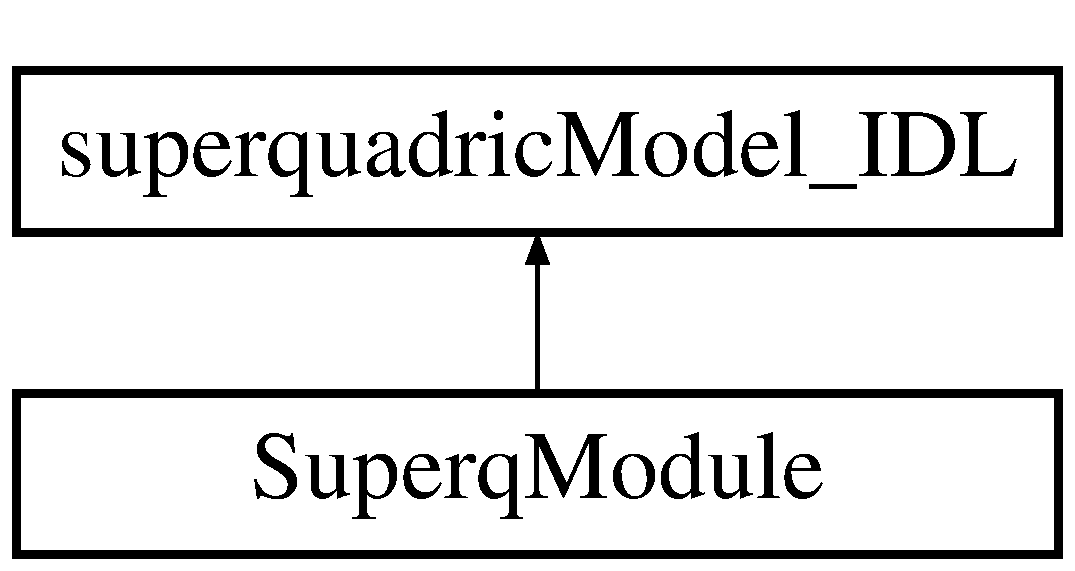
\includegraphics[height=2.000000cm]{classSuperqModule}
\end{center}
\end{figure}
\subsection*{Public Member Functions}
\begin{DoxyCompactItemize}
\item 
double \hyperlink{classSuperqModule_aeec20285d89c1542d1b91c05c0f82539}{get\-Period} ()
\begin{DoxyCompactList}\small\item\em Get period function of R\-F module. \end{DoxyCompactList}\item 
bool \hyperlink{classSuperqModule_adba43b8815167f66e940bd80ab944af3}{update\-Module} ()\label{classSuperqModule_adba43b8815167f66e940bd80ab944af3}

\begin{DoxyCompactList}\small\item\em update\-Module function of R\-F module \end{DoxyCompactList}\item 
bool \hyperlink{classSuperqModule_a99527edc64196d4a9136416331fd5dd1}{configure} (yarp\-::os\-::\-Resource\-Finder \&rf)\label{classSuperqModule_a99527edc64196d4a9136416331fd5dd1}

\begin{DoxyCompactList}\small\item\em configure function of R\-F module \end{DoxyCompactList}\item 
bool \hyperlink{classSuperqModule_aca14ea8a02d8dbdef9a023da4c336891}{interrupt\-Module} ()\label{classSuperqModule_aca14ea8a02d8dbdef9a023da4c336891}

\begin{DoxyCompactList}\small\item\em interrupt module function of R\-F module \end{DoxyCompactList}\item 
bool \hyperlink{classSuperqModule_a6f88e21fe14a124919ffb07e26c04d15}{close} ()\label{classSuperqModule_a6f88e21fe14a124919ffb07e26c04d15}

\begin{DoxyCompactList}\small\item\em close function of R\-F module \end{DoxyCompactList}\item 
bool \hyperlink{classSuperqModule_a045733615dbe0c97f714dde4ea47a164}{config\-On\-Off} (yarp\-::os\-::\-Resource\-Finder \&rf)\label{classSuperqModule_a045733615dbe0c97f714dde4ea47a164}

\begin{DoxyCompactList}\small\item\em Configure all on/off options. \end{DoxyCompactList}\item 
bool \hyperlink{classSuperqModule_abe9bafeec746eb23da8f89cada86849e}{config\-Filter} (yarp\-::os\-::\-Resource\-Finder \&rf)\label{classSuperqModule_abe9bafeec746eb23da8f89cada86849e}

\begin{DoxyCompactList}\small\item\em Configure point cloud filter options. \end{DoxyCompactList}\item 
bool \hyperlink{classSuperqModule_a706feb064c09186585a97422603e6278}{config\-Filter\-Superq} (yarp\-::os\-::\-Resource\-Finder \&rf)\label{classSuperqModule_a706feb064c09186585a97422603e6278}

\begin{DoxyCompactList}\small\item\em Configure superquadric filter options. \end{DoxyCompactList}\item 
bool \hyperlink{classSuperqModule_aa27116ca1ef35ae86459aad82f4c53cb}{config\-Services} (yarp\-::os\-::\-Resource\-Finder \&rf)\label{classSuperqModule_aa27116ca1ef35ae86459aad82f4c53cb}

\begin{DoxyCompactList}\small\item\em Open ports for communication. \end{DoxyCompactList}\item 
bool \hyperlink{classSuperqModule_a36f445a18edc230bcd119b098143204f}{config\-Superq} (yarp\-::os\-::\-Resource\-Finder \&rf)\label{classSuperqModule_a36f445a18edc230bcd119b098143204f}

\begin{DoxyCompactList}\small\item\em Configure superquadric computation otpions. \end{DoxyCompactList}\item 
bool \hyperlink{classSuperqModule_ac92cfd73d4a1e08013051681ccb2e687}{config\-Viewer} (yarp\-::os\-::\-Resource\-Finder \&rf)\label{classSuperqModule_ac92cfd73d4a1e08013051681ccb2e687}

\begin{DoxyCompactList}\small\item\em Configure visualization options. \end{DoxyCompactList}\item 
void \hyperlink{classSuperqModule_ada9aa974cf680e4f6e5507c2dc463856}{save\-Superq} ()\label{classSuperqModule_ada9aa974cf680e4f6e5507c2dc463856}

\begin{DoxyCompactList}\small\item\em Save computed superquadric. \end{DoxyCompactList}\item 
bool \hyperlink{classSuperqModule_a90826fc53859ecf126f22a2569611b2c}{set\-\_\-save\-\_\-points} (const std\-::string \&entry)
\begin{DoxyCompactList}\small\item\em Set if to save or not the used point cloud. \end{DoxyCompactList}\item 
std\-::string \hyperlink{classSuperqModule_adfeeea091edd0d32d388b072f4fc9d93}{get\-\_\-save\-\_\-points} ()
\begin{DoxyCompactList}\small\item\em Get if the used point cloud is saved or not. \end{DoxyCompactList}\item 
bool \hyperlink{classSuperqModule_a0e6af855b1a0f647ff4b9deca973c55d}{read\-Point\-Cloud} ()\label{classSuperqModule_a0e6af855b1a0f647ff4b9deca973c55d}

\begin{DoxyCompactList}\small\item\em In offline mode, read the point cloud from a txt file. \end{DoxyCompactList}\item 
virtual yarp\-::os\-::\-Property \hyperlink{classsuperquadricModel__IDL_a10039bb93445066d9dd29d8f6c9ef6c5}{get\-\_\-superq} (const std\-::vector$<$ yarp\-::sig\-::\-Vector $>$ \&point\-\_\-cloud, const bool filtered\-\_\-or\-\_\-not, const bool reset\-\_\-or\-\_\-not)
\begin{DoxyCompactList}\small\item\em Get the parameters of the reconstructed superquadric. \end{DoxyCompactList}\item 
virtual bool {\bfseries read} (yarp\-::os\-::\-Connection\-Reader \&connection)\label{classsuperquadricModel__IDL_ac72a24dddca13978d7adcd5cf4f40b1f}

\item 
virtual std\-::vector$<$ std\-::string $>$ {\bfseries help} (const std\-::string \&function\-Name=\char`\"{}-\/-\/all\char`\"{})\label{classsuperquadricModel__IDL_a263ca3dc1c7a21cc3ac40caadc95cf3d}

\end{DoxyCompactItemize}
\subsection*{Protected Member Functions}
\begin{DoxyCompactItemize}
\item 
bool {\bfseries attach} (yarp\-::os\-::\-Rpc\-Server \&source)\label{classSuperqModule_a561e16c3b62e17a2fb96193c079bd970}

\item 
bool \hyperlink{classSuperqModule_ae9f0cfead2c367e4c3aa25292b5c42c6}{set\-\_\-tag\-\_\-file} (const std\-::string \&tag\-\_\-file)
\begin{DoxyCompactList}\small\item\em Set a tag name for saving the superquadric. \end{DoxyCompactList}\item 
std\-::string \hyperlink{classSuperqModule_ac5475155a5a1b05e5fdef54699cef1a6}{get\-\_\-tag\-\_\-file} ()
\begin{DoxyCompactList}\small\item\em Get the tag name used for saving the superquadric. \end{DoxyCompactList}\item 
std\-::string \hyperlink{classSuperqModule_a89be4778051c4dd19339021448f89b41}{get\-\_\-visualization} ()
\begin{DoxyCompactList}\small\item\em Return if visualization is on or off. \end{DoxyCompactList}\item 
bool \hyperlink{classSuperqModule_ae4fc54ad89b3ee72ab5ea8c8b5065866}{set\-\_\-visualization} (const std\-::string \&e)
\begin{DoxyCompactList}\small\item\em Set if visualization is on or off. \end{DoxyCompactList}\item 
yarp\-::os\-::\-Property \hyperlink{classSuperqModule_a4a28afabfeac67e807dcc32845b41e0c}{get\-\_\-superq} (const std\-::vector$<$ yarp\-::sig\-::\-Vector $>$ \&blob)
\begin{DoxyCompactList}\small\item\em Return the computed superquadric, given the 2\-D blob of the object. \end{DoxyCompactList}\item 
bool \hyperlink{classSuperqModule_aa5a3fb751dd83d96004fceebab14c139}{send\-\_\-point\-\_\-clouds} (const std\-::vector$<$ yarp\-::sig\-::\-Vector $>$ \&p)
\begin{DoxyCompactList}\small\item\em Get the point cloud for computing the superquadric. \end{DoxyCompactList}\item 
bool \hyperlink{classSuperqModule_ae234e2b5b715e64ef928905964660122}{reset\-\_\-filter} ()
\begin{DoxyCompactList}\small\item\em Reset median filter for improving superquadric estimation. \end{DoxyCompactList}\item 
yarp\-::os\-::\-Property \hyperlink{classSuperqModule_aa6825617672381dcf3eb81dc643f0aaa}{get\-\_\-superq\-\_\-filtered} ()
\begin{DoxyCompactList}\small\item\em Return the filtered superquadric. \end{DoxyCompactList}\item 
yarp\-::os\-::\-Property \hyperlink{classSuperqModule_ae2935a960968a6354462a728e16d60b0}{fill\-Property} (const yarp\-::sig\-::\-Vector \&sol)
\begin{DoxyCompactList}\small\item\em Property fill the property with the superquadric solution. \end{DoxyCompactList}\item 
bool \hyperlink{classSuperqModule_a408203d0119443fb61544f84dafff8a4}{set\-\_\-points\-\_\-filtering} (const std\-::string \&entry)
\begin{DoxyCompactList}\small\item\em Set if to filter or not the point cloud. \end{DoxyCompactList}\item 
std\-::string \hyperlink{classSuperqModule_a60c8ff17436cc55a3e9b704dd6c2529b}{get\-\_\-points\-\_\-filtering} ()
\begin{DoxyCompactList}\small\item\em Get if the point cloud is filtered or not. \end{DoxyCompactList}\item 
bool \hyperlink{classSuperqModule_a902d4a48d1a919ff9d9b1f7d1c132577}{set\-\_\-superq\-\_\-filtering} (const std\-::string \&entry)
\begin{DoxyCompactList}\small\item\em Set if to filter or not the superquadric. \end{DoxyCompactList}\item 
std\-::string \hyperlink{classSuperqModule_a66cb1b371b92687d851b5ca23174198b}{get\-\_\-superq\-\_\-filtering} ()
\begin{DoxyCompactList}\small\item\em Get if the superquadric is filtered or not. \end{DoxyCompactList}\item 
yarp\-::os\-::\-Property \hyperlink{classSuperqModule_a18822e0a99dc0b13479f20960c577fb9}{get\-\_\-options} (const std\-::string \&field)
\begin{DoxyCompactList}\small\item\em Get options of a given field\-: visualization, optimization, filtering. \end{DoxyCompactList}\item 
bool \hyperlink{classSuperqModule_a32ccf59ac0572ca77883237dd2d12890}{set\-\_\-options} (const yarp\-::os\-::\-Property \&new\-Options, const std\-::string \&field)
\begin{DoxyCompactList}\small\item\em Set options of specified field\-: visualization, optimization, filtering. \end{DoxyCompactList}\item 
bool \hyperlink{classSuperqModule_aa00f3e123ab12a0c65f864f2900c36e4}{set\-\_\-object\-\_\-class} (const std\-::string \&objclass)
\begin{DoxyCompactList}\small\item\em Set object class for improving superquadric estimation. \end{DoxyCompactList}\end{DoxyCompactItemize}
\subsection*{Protected Attributes}
\begin{DoxyCompactItemize}
\item 
int {\bfseries r}\label{classSuperqModule_ada2b94883ea2a69f9fab8cb045a5a138}

\item 
int {\bfseries g}\label{classSuperqModule_a1d40ba1a934cd176b0365116597814da}

\item 
int {\bfseries b}\label{classSuperqModule_a048daff404a4f8d8dd83072f5e7675cd}

\item 
int {\bfseries count}\label{classSuperqModule_a4fbfa7613a6f89c61454b61acf288b9f}

\item 
int {\bfseries rate}\label{classSuperqModule_aa778e1c9f9b6627b72bafe1c45e097b9}

\item 
int {\bfseries rate\-\_\-vis}\label{classSuperqModule_ad0dab1b5c69a32f877eac1ca745a0cbc}

\item 
std\-::string {\bfseries tag\-\_\-file}\label{classSuperqModule_a06b5f43aeaa26b5ca5961670f8883ab4}

\item 
std\-::string {\bfseries home\-Context\-Path}\label{classSuperqModule_aa767064e88d01bc7cd8fb2038c63e150}

\item 
yarp\-::os\-::\-Const\-String {\bfseries point\-Cloud\-File\-Name}\label{classSuperqModule_aa719adf35eb593b75e0f0930aa18a4f7}

\item 
std\-::string {\bfseries output\-File\-Name}\label{classSuperqModule_aac8cd7786df2bc4aeb0f7290807c4c49}

\item 
std\-::vector$<$ cv\-::\-Point $>$ {\bfseries contour}\label{classSuperqModule_a2a3cbd0eb9042671dbbc457f5cb25c29}

\item 
std\-::deque$<$ yarp\-::sig\-::\-Vector $>$ {\bfseries points}\label{classSuperqModule_a9d894dfd7e6564ee41a98619c8178584}

\item 
std\-::deque$<$ yarp\-::sig\-::\-Vector $>$ {\bfseries points\-\_\-aux}\label{classSuperqModule_a94cb68f67f8c51a188e12db5fad27565}

\item 
std\-::deque$<$ cv\-::\-Point $>$ {\bfseries blob\-\_\-points}\label{classSuperqModule_a571d62b869e77e87b5fad6a13a72f813}

\item 
double {\bfseries radius}\label{classSuperqModule_a0751c095220723cf7d8b25b5d45a92e1}

\item 
int {\bfseries nn\-Threshold}\label{classSuperqModule_ab7798766f824ed28f1f4dae8a3f1356c}

\item 
int {\bfseries num\-Vertices}\label{classSuperqModule_a9cc4835f5280e71876b76331288b8dc2}

\item 
int {\bfseries median\-\_\-order}\label{classSuperqModule_ae2d1a7a9301e43d148afda36fddd87b4}

\item 
int {\bfseries min\-\_\-median\-\_\-order}\label{classSuperqModule_a96b534ae428e744f2b44d35866490fdc}

\item 
int {\bfseries max\-\_\-median\-\_\-order}\label{classSuperqModule_a1d1b6f621d446969d9a8aa9abfafa7f9}

\item 
int {\bfseries new\-\_\-median\-\_\-order}\label{classSuperqModule_a1409f49f4c5824ec604ce214654d3e22}

\item 
bool {\bfseries filter\-\_\-points}\label{classSuperqModule_aa1bc1b1b7d3ef1b287d0c8d15d9a51bc}

\item 
bool {\bfseries fixed\-\_\-window}\label{classSuperqModule_a07ff8af914d2f3b5ae9fbc03b94954e7}

\item 
bool {\bfseries filter\-\_\-superq}\label{classSuperqModule_a3e824c0b36749d3e9d2ff755004b7472}

\item 
std\-::string {\bfseries what\-\_\-to\-\_\-plot}\label{classSuperqModule_a1f1963d5a8947368cec96d4fbcc3ec79}

\item 
double {\bfseries threshold\-\_\-median}\label{classSuperqModule_a226a730b20160c8e6483bd3b1064a7bc}

\item 
double {\bfseries min\-\_\-norm\-\_\-vel}\label{classSuperqModule_ace8ceaaf035427634c78f3d720ab2432}

\item 
bool {\bfseries mode\-\_\-online}\label{classSuperqModule_adfab63f5b7aad436d9833898ea23602a}

\item 
bool {\bfseries visualization\-\_\-on}\label{classSuperqModule_aecdc7d85514cc472b7a91982d6b1f58d}

\item 
bool {\bfseries go\-\_\-on}\label{classSuperqModule_a46bddbc5530c3086005ad07281bc5ae9}

\item 
bool {\bfseries reset}\label{classSuperqModule_ad3f77b480fd86b554fabf882c090ddc1}

\item 
bool {\bfseries save\-\_\-points}\label{classSuperqModule_a67a8bc8f0d0464efc29caf5465f256e6}

\item 
double {\bfseries tol}\label{classSuperqModule_ad4843804d3d340b725debf434e5347b5}

\item 
double {\bfseries sum}\label{classSuperqModule_a01f96b54badeaf38908355577586a4c0}

\item 
double {\bfseries max\-\_\-cpu\-\_\-time}\label{classSuperqModule_aace6a0e5aa42c5e376a5e60397a4dcea}

\item 
int {\bfseries acceptable\-\_\-iter}\label{classSuperqModule_ab3c64f8ffe227d91ab3fcc8983589b3a}

\item 
int {\bfseries max\-\_\-iter}\label{classSuperqModule_ae130c3d3d0ac884336761ded94731f1b}

\item 
int {\bfseries optimizer\-\_\-points}\label{classSuperqModule_ae796a494cc0be47bf8888e9f876784dc}

\item 
std\-::string {\bfseries mu\-\_\-strategy}\label{classSuperqModule_a29a3eb467fb15cb219b43c70a8cfda8a}

\item 
std\-::string {\bfseries nlp\-\_\-scaling\-\_\-method}\label{classSuperqModule_a01f9c7e0ec759b78c782483aaf2f0085}

\item 
yarp\-::sig\-::\-Vector {\bfseries x}\label{classSuperqModule_a8b845bdc0c6d35d90141968502ca9d96}

\item 
yarp\-::sig\-::\-Vector {\bfseries x\-\_\-filtered}\label{classSuperqModule_adb96b7bb58edc83b70dcd4781b51130a}

\item 
double {\bfseries t\-\_\-superq}\label{classSuperqModule_a981bafe724d09df7beb3c10fa96a8980}

\item 
std\-::deque$<$ double $>$ {\bfseries times\-\_\-superq}\label{classSuperqModule_a28517e736a16c5e7dfde3bcbec6bf5fd}

\item 
double {\bfseries t\-\_\-vis}\label{classSuperqModule_ac4b02568e69c9ed84739bb252a31def6}

\item 
std\-::deque$<$ double $>$ {\bfseries times\-\_\-vis}\label{classSuperqModule_af8194f823d1dfc5072988680d71aab08}

\item 
yarp\-::os\-::\-Buffered\-Port\\*
$<$ yarp\-::sig\-::\-Image\-Of\\*
$<$ yarp\-::sig\-::\-Pixel\-Rgb $>$ $>$ {\bfseries port\-Img\-In}\label{classSuperqModule_aff224bd8fb7b12d73b2060b38f7a8718}

\item 
yarp\-::os\-::\-Buffered\-Port\\*
$<$ yarp\-::os\-::\-Property $>$ {\bfseries port\-Superq}\label{classSuperqModule_ac73ad3c50ea4fe58e35a722c37a7f99e}

\item 
yarp\-::os\-::\-Rpc\-Server {\bfseries port\-Rpc}\label{classSuperqModule_ab44a4843a8cb533d80d55df985b11448}

\item 
int {\bfseries vis\-\_\-points}\label{classSuperqModule_ae8e5d7e83ef5cd80a44ce6a3bcc74cd7}

\item 
int {\bfseries vis\-\_\-step}\label{classSuperqModule_a73aa4f6c8c4c9142fb5456c9cdaaf6b6}

\item 
std\-::string {\bfseries eye}\label{classSuperqModule_a016da49606647c049c4b857a32c633c6}

\item 
yarp\-::sig\-::\-Matrix {\bfseries R}\label{classSuperqModule_ab0570fcea5cbee6364f780cca614164d}

\item 
yarp\-::sig\-::\-Matrix {\bfseries H}\label{classSuperqModule_acf23ebc65162db020fd4e25ca73ea165}

\item 
yarp\-::sig\-::\-Matrix {\bfseries K}\label{classSuperqModule_ac6ee7467d82e835c0d1b2e35236e4aaf}

\item 
yarp\-::sig\-::\-Vector {\bfseries point}\label{classSuperqModule_a80128e303c0d59016e41493ca50cc94e}

\item 
yarp\-::sig\-::\-Vector {\bfseries point1}\label{classSuperqModule_ab8daf379295df5a47ced6f06acfe0df9}

\item 
yarp\-::sig\-::\-Vector {\bfseries point2\-D}\label{classSuperqModule_a8839fda8369d4e2e73714cc1db6e0f5e}

\item 
std\-::deque$<$ int $>$ {\bfseries Color}\label{classSuperqModule_a15f7523202cf192d71f188db2647e50c}

\item 
yarp\-::dev\-::\-Poly\-Driver {\bfseries Gaze\-Ctrl}\label{classSuperqModule_a1ce22879df6c4586ed72a3e3b67609bb}

\item 
yarp\-::dev\-::\-I\-Gaze\-Control $\ast$ {\bfseries igaze}\label{classSuperqModule_a00ea631bed0909310e2e505f0aca688f}

\item 
yarp\-::os\-::\-Resource\-Finder $\ast$ {\bfseries rf}\label{classSuperqModule_ac781b86f89aab354c250c17cff49c2d8}

\item 
double {\bfseries t}\label{classSuperqModule_a7246f334af9922695d716a5afb4ce89e}

\item 
double {\bfseries t0}\label{classSuperqModule_aa0788b39ee666e4cd09ea4c59421dc24}

\item 
std\-::deque$<$ std\-::string $>$ {\bfseries advanced\-\_\-params}\label{classSuperqModule_aa45e8a64fbe20bc54d9f303369a618aa}

\item 
yarp\-::os\-::\-Mutex {\bfseries mutex}\label{classSuperqModule_a04543bfe968184ff3ee55905c90f12ac}

\item 
yarp\-::os\-::\-Mutex {\bfseries mutex\-\_\-shared}\label{classSuperqModule_aa6671c2457e2044f3823d671a9b7e6ea}

\item 
std\-::string {\bfseries object\-\_\-class}\label{classSuperqModule_ae26497c030a1ecd16b98096c5842f383}

\item 
Superq\-Computation $\ast$ {\bfseries superq\-Com}\label{classSuperqModule_adab3d841bcfd52387bb6dd861fddf424}

\item 
\hyperlink{classSuperqVisualization}{Superq\-Visualization} $\ast$ {\bfseries superq\-Vis}\label{classSuperqModule_a91b35d4f88a0bfda1bb6f0bcfa6976b1}

\item 
yarp\-::os\-::\-Property {\bfseries filter\-\_\-points\-\_\-par}\label{classSuperqModule_a86c20777e5607bb326216605bab0e222}

\item 
yarp\-::os\-::\-Property {\bfseries filter\-\_\-superq\-\_\-par}\label{classSuperqModule_ac9c130b5960c724aed615bbf6ac17b50}

\item 
yarp\-::os\-::\-Property {\bfseries ipopt\-\_\-par}\label{classSuperqModule_a6469063a5f34843741f727696d1803e1}

\item 
yarp\-::sig\-::\-Image\-Of\\*
$<$ yarp\-::sig\-::\-Pixel\-Rgb $>$ $\ast$ {\bfseries img\-In}\label{classSuperqModule_ae0c421e0a3f04758c2e75a06a2fa83b7}

\end{DoxyCompactItemize}


\subsection{Detailed Description}
The \hyperlink{classSuperqModule}{Superq\-Module} class handle the superquadric computation and visualization, the point cloud and superquadric filtering and the interaction with the user. 

It is used to set all the parameters (offline and online) and to launch all the thread for superquadric computation and visualization. 

Definition at line 40 of file superq\-Module.\-h.



\subsection{Member Function Documentation}
\index{Superq\-Module@{Superq\-Module}!fill\-Property@{fill\-Property}}
\index{fill\-Property@{fill\-Property}!SuperqModule@{Superq\-Module}}
\subsubsection[{fill\-Property}]{\setlength{\rightskip}{0pt plus 5cm}Property Superq\-Module\-::fill\-Property (
\begin{DoxyParamCaption}
\item[{const yarp\-::sig\-::\-Vector \&}]{sol}
\end{DoxyParamCaption}
)\hspace{0.3cm}{\ttfamily [protected]}}\label{classSuperqModule_ae2935a960968a6354462a728e16d60b0}


Property fill the property with the superquadric solution. 


\begin{DoxyParams}{Parameters}
{\em sol} & is a Vector of the computed superquadric \\
\hline
\end{DoxyParams}
\begin{DoxyReturn}{Returns}
a Property with the solution 
\end{DoxyReturn}


Definition at line 195 of file superq\-Module.\-cpp.


\begin{DoxyCode}
196 \{
197     Property superq;
198 
199     Bottle bottle;
200     Bottle &b1=bottle.addList();
201     b1.addDouble(sol[0]); b1.addDouble(sol[1]); b1.addDouble(sol[2]);
202     superq.put(\textcolor{stringliteral}{"dimensions"}, bottle.get(0));
203 
204     Bottle &b2=bottle.addList();
205     b2.addDouble(sol[3]); b2.addDouble(sol[4]);
206     superq.put(\textcolor{stringliteral}{"exponents"}, bottle.get(1));
207 
208     Bottle &b3=bottle.addList();
209     b3.addDouble(sol[5]); b3.addDouble(sol[6]); b3.addDouble(sol[7]);
210     superq.put(\textcolor{stringliteral}{"center"}, bottle.get(2));
211 
212     Bottle &b4=bottle.addList();
213     Vector orient=dcm2axis(euler2dcm(sol.subVector(8,10)));
214     b4.addDouble(orient[0]); b4.addDouble(orient[1]); b4.addDouble(orient[2]); b4.addDouble(orient[3]);
215     superq.put(\textcolor{stringliteral}{"orientation"}, bottle.get(3));
216     \textcolor{keywordflow}{return} superq;
217 \}
\end{DoxyCode}
\index{Superq\-Module@{Superq\-Module}!get\-\_\-options@{get\-\_\-options}}
\index{get\-\_\-options@{get\-\_\-options}!SuperqModule@{Superq\-Module}}
\subsubsection[{get\-\_\-options}]{\setlength{\rightskip}{0pt plus 5cm}Property Superq\-Module\-::get\-\_\-options (
\begin{DoxyParamCaption}
\item[{const std\-::string \&}]{field}
\end{DoxyParamCaption}
)\hspace{0.3cm}{\ttfamily [protected]}, {\ttfamily [virtual]}}\label{classSuperqModule_a18822e0a99dc0b13479f20960c577fb9}


Get options of a given field\-: visualization, optimization, filtering. 


\begin{DoxyParams}{Parameters}
{\em field} & is one of the field of options \\
\hline
\end{DoxyParams}
\begin{DoxyReturn}{Returns}
property with the options of interested 
\end{DoxyReturn}


Reimplemented from \hyperlink{classsuperquadricModel__IDL_a50b388a29852f9d8b57a0bbb276d4675}{superquadric\-Model\-\_\-\-I\-D\-L}.



Definition at line 338 of file superq\-Module.\-cpp.


\begin{DoxyCode}
339 \{
340     Property advOptions;
341     \textcolor{keywordflow}{if} (field==\textcolor{stringliteral}{"points\_filter"})
342         advOptions=superqCom->getPointsFilterPar();
343     \textcolor{keywordflow}{else} \textcolor{keywordflow}{if} (field==\textcolor{stringliteral}{"superq\_filter"})
344         advOptions=superqCom->getSuperqFilterPar();
345     \textcolor{keywordflow}{else} \textcolor{keywordflow}{if} (field==\textcolor{stringliteral}{"optimization"})
346         advOptions=superqCom->getIpoptPar();
347     \textcolor{keywordflow}{else} \textcolor{keywordflow}{if} (field==\textcolor{stringliteral}{"visualization"})
348         advOptions=superqVis->getPar();
349     \textcolor{keywordflow}{else} \textcolor{keywordflow}{if} (field==\textcolor{stringliteral}{"statistics"})
350     \{
351         advOptions.put(\textcolor{stringliteral}{"average\_computation\_time"}, t\_superq);
352         advOptions.put(\textcolor{stringliteral}{"average\_visualization\_time"}, t\_vis);
353     \}       
354 
355     \textcolor{keywordflow}{return} advOptions;
356 \}
\end{DoxyCode}
\index{Superq\-Module@{Superq\-Module}!get\-\_\-points\-\_\-filtering@{get\-\_\-points\-\_\-filtering}}
\index{get\-\_\-points\-\_\-filtering@{get\-\_\-points\-\_\-filtering}!SuperqModule@{Superq\-Module}}
\subsubsection[{get\-\_\-points\-\_\-filtering}]{\setlength{\rightskip}{0pt plus 5cm}string Superq\-Module\-::get\-\_\-points\-\_\-filtering (
\begin{DoxyParamCaption}
{}
\end{DoxyParamCaption}
)\hspace{0.3cm}{\ttfamily [protected]}, {\ttfamily [virtual]}}\label{classSuperqModule_a60c8ff17436cc55a3e9b704dd6c2529b}


Get if the point cloud is filtered or not. 

\begin{DoxyReturn}{Returns}
\char`\"{}on\char`\"{} or \char`\"{}off\char`\"{} 
\end{DoxyReturn}


Reimplemented from \hyperlink{classsuperquadricModel__IDL_aa490ebcf39414aaaae41d5095267abb9}{superquadric\-Model\-\_\-\-I\-D\-L}.



Definition at line 250 of file superq\-Module.\-cpp.


\begin{DoxyCode}
251 \{
252     \textcolor{keywordflow}{if} (filter\_points)
253     \{
254         \textcolor{keywordflow}{return} \textcolor{stringliteral}{"on"};
255     \}
256     \textcolor{keywordflow}{else}
257     \{
258         \textcolor{keywordflow}{return} \textcolor{stringliteral}{"off"};
259     \}
260 \}
\end{DoxyCode}
\index{Superq\-Module@{Superq\-Module}!get\-\_\-save\-\_\-points@{get\-\_\-save\-\_\-points}}
\index{get\-\_\-save\-\_\-points@{get\-\_\-save\-\_\-points}!SuperqModule@{Superq\-Module}}
\subsubsection[{get\-\_\-save\-\_\-points}]{\setlength{\rightskip}{0pt plus 5cm}string Superq\-Module\-::get\-\_\-save\-\_\-points (
\begin{DoxyParamCaption}
{}
\end{DoxyParamCaption}
)\hspace{0.3cm}{\ttfamily [virtual]}}\label{classSuperqModule_adfeeea091edd0d32d388b072f4fc9d93}


Get if the used point cloud is saved or not. 

\begin{DoxyReturn}{Returns}
\char`\"{}on\char`\"{} or \char`\"{}off\char`\"{} 
\end{DoxyReturn}


Reimplemented from \hyperlink{classsuperquadricModel__IDL_a4b101fe118a1ee912468562bde0b0df4}{superquadric\-Model\-\_\-\-I\-D\-L}.



Definition at line 312 of file superq\-Module.\-cpp.


\begin{DoxyCode}
313 \{
314     \textcolor{keywordflow}{if} (save\_points)
315     \{
316         \textcolor{keywordflow}{return} \textcolor{stringliteral}{"on"};
317     \}
318     \textcolor{keywordflow}{else}
319     \{
320         \textcolor{keywordflow}{return} \textcolor{stringliteral}{"off"};
321     \}
322 \}
\end{DoxyCode}
\index{Superq\-Module@{Superq\-Module}!get\-\_\-superq@{get\-\_\-superq}}
\index{get\-\_\-superq@{get\-\_\-superq}!SuperqModule@{Superq\-Module}}
\subsubsection[{get\-\_\-superq}]{\setlength{\rightskip}{0pt plus 5cm}virtual yarp\-::os\-::\-Property superquadric\-Model\-\_\-\-I\-D\-L\-::get\-\_\-superq (
\begin{DoxyParamCaption}
\item[{const std\-::vector$<$ yarp\-::sig\-::\-Vector $>$ \&}]{point\-\_\-cloud, }
\item[{const bool}]{filtered\-\_\-or\-\_\-not, }
\item[{const bool}]{reset\-\_\-or\-\_\-not}
\end{DoxyParamCaption}
)\hspace{0.3cm}{\ttfamily [virtual]}, {\ttfamily [inherited]}}\label{classsuperquadricModel__IDL_a10039bb93445066d9dd29d8f6c9ef6c5}


Get the parameters of the reconstructed superquadric. 


\begin{DoxyParams}{Parameters}
{\em point\-\_\-cloud} & is the 3\-D point cloud of the object we want to model with the superquadric, for instance\-: ((100.\-0 102.\-0) (100.\-0 103.\-0) ... ). \\
\hline
{\em filtered\-\_\-or\-\_\-not} & is a bool variable specifing if we want the superquadric to be filtered (true/1) or not (false/0). \\
\hline
{\em reset\-\_\-or\-\_\-not} & is a bool variable specifing if we want to reset the superquadric filtered (if enabled) or not. \\
\hline
\end{DoxyParams}
\begin{DoxyReturn}{Returns}
the 12 parameters (x0, .. x11) of the current superquadric. In particular, the parameters are grouped in a Property as follows\-: \char`\"{}dimensions\char`\"{} (x0, x1, x2) are the three semi-\/axes lenghts; \char`\"{}exponents\char`\"{} (x3 and x4) are the exponents, responsible for the superquadric shape; \char`\"{}center\char`\"{}(x5, x6, x7) contains the coordinate of the superquadric center; and \char`\"{}orientation\char`\"{} (x8, x9, 10, x11) is the axis-\/angle representation obtained from the Euler angles. 
\end{DoxyReturn}
\index{Superq\-Module@{Superq\-Module}!get\-\_\-superq@{get\-\_\-superq}}
\index{get\-\_\-superq@{get\-\_\-superq}!SuperqModule@{Superq\-Module}}
\subsubsection[{get\-\_\-superq}]{\setlength{\rightskip}{0pt plus 5cm}Property Superq\-Module\-::get\-\_\-superq (
\begin{DoxyParamCaption}
\item[{const std\-::vector$<$ yarp\-::sig\-::\-Vector $>$ \&}]{blob}
\end{DoxyParamCaption}
)\hspace{0.3cm}{\ttfamily [protected]}}\label{classSuperqModule_a4a28afabfeac67e807dcc32845b41e0c}


Return the computed superquadric, given the 2\-D blob of the object. 


\begin{DoxyParams}{Parameters}
{\em blob} & is the 2\-D blob of the object \\
\hline
\end{DoxyParams}
\begin{DoxyReturn}{Returns}
a property with the estimated superquadric 
\end{DoxyReturn}


Definition at line 99 of file superq\-Module.\-cpp.


\begin{DoxyCode}
100 \{
101     Property superq;
102 
103     LockGuard lg(mutex);
104     \textcolor{comment}{//LockGuard lg(mutex\_shared);}
105 
106     superqCom->setPar(\textcolor{stringliteral}{"object\_class"}, object\_class);
107 
108     superqCom->setPar(\textcolor{stringliteral}{"one\_shot"}, \textcolor{stringliteral}{"on"});
109 
110     deque<Vector> p\_aux;
111     
112     \textcolor{keywordflow}{for} (\textcolor{keywordtype}{size\_t} i=0; i<p.size(); i++)
113         p\_aux.push\_back(p[i]);
114 
115     superqCom->sendPoints(p\_aux);
116 
117     \textcolor{comment}{//superqCom->step();}
118     superqCom->run();
119 
120     Vector sol(11,0.0);
121     sol=superqCom->getSolution(0);
122 
123     superqCom->setPar(\textcolor{stringliteral}{"one\_shot"}, \textcolor{stringliteral}{"off"});
124     p\_aux.clear();
125     superqCom->sendPoints(p\_aux);
126 
127     superq=fillProperty(sol);
128 
129     \textcolor{keywordflow}{return} superq;
130 \}
\end{DoxyCode}
\index{Superq\-Module@{Superq\-Module}!get\-\_\-superq\-\_\-filtered@{get\-\_\-superq\-\_\-filtered}}
\index{get\-\_\-superq\-\_\-filtered@{get\-\_\-superq\-\_\-filtered}!SuperqModule@{Superq\-Module}}
\subsubsection[{get\-\_\-superq\-\_\-filtered}]{\setlength{\rightskip}{0pt plus 5cm}Property Superq\-Module\-::get\-\_\-superq\-\_\-filtered (
\begin{DoxyParamCaption}
{}
\end{DoxyParamCaption}
)\hspace{0.3cm}{\ttfamily [protected]}}\label{classSuperqModule_aa6825617672381dcf3eb81dc643f0aaa}


Return the filtered superquadric. 

\begin{DoxyReturn}{Returns}
a property with the filtered superquadric 
\end{DoxyReturn}


Definition at line 177 of file superq\-Module.\-cpp.


\begin{DoxyCode}
178 \{
179     \textcolor{comment}{//LockGuard lg(mutex);}
180     Property superq;
181     Vector sol(11,0.0);
182     sol=superqCom->getSolution(1);
183 
184     superqCom->setPar(\textcolor{stringliteral}{"one\_shot"}, \textcolor{stringliteral}{"off"});
185     deque<Vector> p\_aux;
186     p\_aux.clear();
187     superqCom->sendPoints(p\_aux);
188 
189     superq=fillProperty(sol);
190 
191     \textcolor{keywordflow}{return} superq;
192 \}
\end{DoxyCode}
\index{Superq\-Module@{Superq\-Module}!get\-\_\-superq\-\_\-filtering@{get\-\_\-superq\-\_\-filtering}}
\index{get\-\_\-superq\-\_\-filtering@{get\-\_\-superq\-\_\-filtering}!SuperqModule@{Superq\-Module}}
\subsubsection[{get\-\_\-superq\-\_\-filtering}]{\setlength{\rightskip}{0pt plus 5cm}string Superq\-Module\-::get\-\_\-superq\-\_\-filtering (
\begin{DoxyParamCaption}
{}
\end{DoxyParamCaption}
)\hspace{0.3cm}{\ttfamily [protected]}, {\ttfamily [virtual]}}\label{classSuperqModule_a66cb1b371b92687d851b5ca23174198b}


Get if the superquadric is filtered or not. 

\begin{DoxyReturn}{Returns}
\char`\"{}on\char`\"{} or \char`\"{}off\char`\"{} 
\end{DoxyReturn}


Reimplemented from \hyperlink{classsuperquadricModel__IDL_af99d29d42b96b8db6c90c5fd48cfb253}{superquadric\-Model\-\_\-\-I\-D\-L}.



Definition at line 299 of file superq\-Module.\-cpp.


\begin{DoxyCode}
300 \{
301     \textcolor{keywordflow}{if} (filter\_superq)
302     \{
303         \textcolor{keywordflow}{return} \textcolor{stringliteral}{"on"};
304     \}
305     \textcolor{keywordflow}{else}
306     \{
307         \textcolor{keywordflow}{return} \textcolor{stringliteral}{"off"};
308     \}
309 \}
\end{DoxyCode}
\index{Superq\-Module@{Superq\-Module}!get\-\_\-tag\-\_\-file@{get\-\_\-tag\-\_\-file}}
\index{get\-\_\-tag\-\_\-file@{get\-\_\-tag\-\_\-file}!SuperqModule@{Superq\-Module}}
\subsubsection[{get\-\_\-tag\-\_\-file}]{\setlength{\rightskip}{0pt plus 5cm}string Superq\-Module\-::get\-\_\-tag\-\_\-file (
\begin{DoxyParamCaption}
{}
\end{DoxyParamCaption}
)\hspace{0.3cm}{\ttfamily [protected]}, {\ttfamily [virtual]}}\label{classSuperqModule_ac5475155a5a1b05e5fdef54699cef1a6}


Get the tag name used for saving the superquadric. 

\begin{DoxyReturn}{Returns}
the currect name of the file used for saving 
\end{DoxyReturn}


Reimplemented from \hyperlink{classsuperquadricModel__IDL_a6d39eaa247aec65fe2bfefbdace4ec85}{superquadric\-Model\-\_\-\-I\-D\-L}.



Definition at line 57 of file superq\-Module.\-cpp.


\begin{DoxyCode}
58 \{
59     \textcolor{keywordflow}{return} tag\_file;
60 \}
\end{DoxyCode}
\index{Superq\-Module@{Superq\-Module}!get\-\_\-visualization@{get\-\_\-visualization}}
\index{get\-\_\-visualization@{get\-\_\-visualization}!SuperqModule@{Superq\-Module}}
\subsubsection[{get\-\_\-visualization}]{\setlength{\rightskip}{0pt plus 5cm}string Superq\-Module\-::get\-\_\-visualization (
\begin{DoxyParamCaption}
{}
\end{DoxyParamCaption}
)\hspace{0.3cm}{\ttfamily [protected]}, {\ttfamily [virtual]}}\label{classSuperqModule_a89be4778051c4dd19339021448f89b41}


Return if visualization is on or off. 

\begin{DoxyReturn}{Returns}
\char`\"{}on\char`\"{} or \char`\"{}off\char`\"{} 
\end{DoxyReturn}


Reimplemented from \hyperlink{classsuperquadricModel__IDL_a5d9f4f0622ba19b60218636dc108ef61}{superquadric\-Model\-\_\-\-I\-D\-L}.



Definition at line 63 of file superq\-Module.\-cpp.


\begin{DoxyCode}
64 \{
65     \textcolor{keywordflow}{if} (visualization\_on)
66         \textcolor{keywordflow}{return} \textcolor{stringliteral}{"on"};
67     \textcolor{keywordflow}{else}
68         \textcolor{keywordflow}{return} \textcolor{stringliteral}{"off"};
69 \}
\end{DoxyCode}
\index{Superq\-Module@{Superq\-Module}!get\-Period@{get\-Period}}
\index{get\-Period@{get\-Period}!SuperqModule@{Superq\-Module}}
\subsubsection[{get\-Period}]{\setlength{\rightskip}{0pt plus 5cm}double Superq\-Module\-::get\-Period (
\begin{DoxyParamCaption}
{}
\end{DoxyParamCaption}
)}\label{classSuperqModule_aeec20285d89c1542d1b91c05c0f82539}


Get period function of R\-F module. 

\begin{DoxyReturn}{Returns}
the period 
\end{DoxyReturn}


Definition at line 384 of file superq\-Module.\-cpp.


\begin{DoxyCode}
385 \{
386     \textcolor{keywordflow}{return} 0.0;
387 \}
\end{DoxyCode}
\index{Superq\-Module@{Superq\-Module}!reset\-\_\-filter@{reset\-\_\-filter}}
\index{reset\-\_\-filter@{reset\-\_\-filter}!SuperqModule@{Superq\-Module}}
\subsubsection[{reset\-\_\-filter}]{\setlength{\rightskip}{0pt plus 5cm}bool Superq\-Module\-::reset\-\_\-filter (
\begin{DoxyParamCaption}
{}
\end{DoxyParamCaption}
)\hspace{0.3cm}{\ttfamily [protected]}}\label{classSuperqModule_ae234e2b5b715e64ef928905964660122}


Reset median filter for improving superquadric estimation. 

\begin{DoxyReturn}{Returns}
true 
\end{DoxyReturn}


Definition at line 169 of file superq\-Module.\-cpp.


\begin{DoxyCode}
170 \{
171     superqCom->resetMedianFilter();
172 
173     \textcolor{keywordflow}{return} \textcolor{keyword}{true};
174 \}
\end{DoxyCode}
\index{Superq\-Module@{Superq\-Module}!send\-\_\-point\-\_\-clouds@{send\-\_\-point\-\_\-clouds}}
\index{send\-\_\-point\-\_\-clouds@{send\-\_\-point\-\_\-clouds}!SuperqModule@{Superq\-Module}}
\subsubsection[{send\-\_\-point\-\_\-clouds}]{\setlength{\rightskip}{0pt plus 5cm}bool Superq\-Module\-::send\-\_\-point\-\_\-clouds (
\begin{DoxyParamCaption}
\item[{const std\-::vector$<$ yarp\-::sig\-::\-Vector $>$ \&}]{p}
\end{DoxyParamCaption}
)\hspace{0.3cm}{\ttfamily [protected]}}\label{classSuperqModule_aa5a3fb751dd83d96004fceebab14c139}


Get the point cloud for computing the superquadric. 


\begin{DoxyParams}{Parameters}
{\em p} & is the point cloud to be acquired \\
\hline
\end{DoxyParams}
\begin{DoxyReturn}{Returns}
true 
\end{DoxyReturn}


Definition at line 133 of file superq\-Module.\-cpp.


\begin{DoxyCode}
134 \{
135     \textcolor{comment}{//LockGuard lg(mutex);}
136 
137     \textcolor{comment}{//LockGuard lg\_shared(mutex\_shared);}
138 
139     \textcolor{keywordtype}{double} t, t\_fin;  
140     
141     t=Time::now();
142 
143     superqCom->setPar(\textcolor{stringliteral}{"object\_class"}, object\_class);
144 
145     yDebug()<<\textcolor{stringliteral}{"Time operations  after set par 1"}<<Time::now() - t;
146 
147     superqCom->setPar(\textcolor{stringliteral}{"one\_shot"}, \textcolor{stringliteral}{"on"});
148 
149     yDebug()<<\textcolor{stringliteral}{"Time operations after set par 2"}<<Time::now() - t;
150 
151     deque<Vector> p\_aux;
152 
153     \textcolor{keywordflow}{for} (\textcolor{keywordtype}{size\_t} i=0; i<p.size(); i++)
154         p\_aux.push\_back(p[i]);
155 
156     superqCom->sendPoints(p\_aux);
157     yDebug()<<\textcolor{stringliteral}{"Time operations send points "}<<Time::now() - t;
158 
159     \textcolor{comment}{//superqCom->step();}
160 
161     t\_fin= Time::now() - t;
162 
163     yDebug()<<\textcolor{stringliteral}{"Time operations  final"}<<t\_fin;
164 
165     \textcolor{keywordflow}{return} \textcolor{keyword}{true};
166 \}
\end{DoxyCode}
\index{Superq\-Module@{Superq\-Module}!set\-\_\-object\-\_\-class@{set\-\_\-object\-\_\-class}}
\index{set\-\_\-object\-\_\-class@{set\-\_\-object\-\_\-class}!SuperqModule@{Superq\-Module}}
\subsubsection[{set\-\_\-object\-\_\-class}]{\setlength{\rightskip}{0pt plus 5cm}bool Superq\-Module\-::set\-\_\-object\-\_\-class (
\begin{DoxyParamCaption}
\item[{const std\-::string \&}]{objclass}
\end{DoxyParamCaption}
)\hspace{0.3cm}{\ttfamily [protected]}}\label{classSuperqModule_aa00f3e123ab12a0c65f864f2900c36e4}


Set object class for improving superquadric estimation. 


\begin{DoxyParams}{Parameters}
{\em objclass} & is the object class (according to the shape) \\
\hline
\end{DoxyParams}
\begin{DoxyReturn}{Returns}
true/false on success/failure 
\end{DoxyReturn}


Definition at line 376 of file superq\-Module.\-cpp.


\begin{DoxyCode}
377 \{
378     object\_class=objclass;
379 
380     \textcolor{keywordflow}{return} \textcolor{keyword}{true};
381 \}
\end{DoxyCode}
\index{Superq\-Module@{Superq\-Module}!set\-\_\-options@{set\-\_\-options}}
\index{set\-\_\-options@{set\-\_\-options}!SuperqModule@{Superq\-Module}}
\subsubsection[{set\-\_\-options}]{\setlength{\rightskip}{0pt plus 5cm}bool Superq\-Module\-::set\-\_\-options (
\begin{DoxyParamCaption}
\item[{const yarp\-::os\-::\-Property \&}]{new\-Options, }
\item[{const std\-::string \&}]{field}
\end{DoxyParamCaption}
)\hspace{0.3cm}{\ttfamily [protected]}, {\ttfamily [virtual]}}\label{classSuperqModule_a32ccf59ac0572ca77883237dd2d12890}


Set options of specified field\-: visualization, optimization, filtering. 


\begin{DoxyParams}{Parameters}
{\em new\-Options} & is a property with the options to be set \\
\hline
{\em field} & is the field of the options to be set \\
\hline
\end{DoxyParams}
\begin{DoxyReturn}{Returns}
true/false on success/failure 
\end{DoxyReturn}


Reimplemented from \hyperlink{classsuperquadricModel__IDL_a575e0b591f07206b0d6c29e5cfeead37}{superquadric\-Model\-\_\-\-I\-D\-L}.



Definition at line 359 of file superq\-Module.\-cpp.


\begin{DoxyCode}
360 \{
361     \textcolor{keywordflow}{if} (field==\textcolor{stringliteral}{"points\_filter"})
362         superqCom->setPointsFilterPar(newOptions, \textcolor{keyword}{false});
363     \textcolor{keywordflow}{else} \textcolor{keywordflow}{if} (field==\textcolor{stringliteral}{"superq\_filter"})
364         superqCom->setSuperqFilterPar(newOptions, \textcolor{keyword}{false});
365     \textcolor{keywordflow}{else} \textcolor{keywordflow}{if} (field==\textcolor{stringliteral}{"optimization"})
366         superqCom->setIpoptPar(newOptions, \textcolor{keyword}{false});
367     \textcolor{keywordflow}{else} \textcolor{keywordflow}{if} (field==\textcolor{stringliteral}{"visualization"})
368         superqVis->setPar(newOptions, \textcolor{keyword}{false});
369     \textcolor{keywordflow}{else}
370         \textcolor{keywordflow}{return} \textcolor{keyword}{false};
371 
372     \textcolor{keywordflow}{return} \textcolor{keyword}{true};
373 \}
\end{DoxyCode}
\index{Superq\-Module@{Superq\-Module}!set\-\_\-points\-\_\-filtering@{set\-\_\-points\-\_\-filtering}}
\index{set\-\_\-points\-\_\-filtering@{set\-\_\-points\-\_\-filtering}!SuperqModule@{Superq\-Module}}
\subsubsection[{set\-\_\-points\-\_\-filtering}]{\setlength{\rightskip}{0pt plus 5cm}bool Superq\-Module\-::set\-\_\-points\-\_\-filtering (
\begin{DoxyParamCaption}
\item[{const std\-::string \&}]{entry}
\end{DoxyParamCaption}
)\hspace{0.3cm}{\ttfamily [protected]}, {\ttfamily [virtual]}}\label{classSuperqModule_a408203d0119443fb61544f84dafff8a4}


Set if to filter or not the point cloud. 


\begin{DoxyParams}{Parameters}
{\em entre} & can be \char`\"{}on\char`\"{} or \char`\"{}off\char`\"{} \\
\hline
\end{DoxyParams}
\begin{DoxyReturn}{Returns}
true/false on success/failure 
\end{DoxyReturn}


Reimplemented from \hyperlink{classsuperquadricModel__IDL_a1a2080d797a81b46b0dffa86b5367e15}{superquadric\-Model\-\_\-\-I\-D\-L}.



Definition at line 220 of file superq\-Module.\-cpp.


\begin{DoxyCode}
221 \{
222     \textcolor{keywordflow}{if} ((entry==\textcolor{stringliteral}{"on"}) || (entry==\textcolor{stringliteral}{"off"}))
223     \{
224         LockGuard lg(mutex);
225         filter\_points=(entry==\textcolor{stringliteral}{"on"});
226         \textcolor{keywordflow}{if} (filter\_points)
227         \{
228             Property options;
229             options.put(\textcolor{stringliteral}{"filter\_radius"}, radius);
230             options.put(\textcolor{stringliteral}{"filter\_nnThreshold"}, nnThreshold);
231             superqCom->setPointsFilterPar(options, \textcolor{keyword}{false});
232             superqCom->setPar(\textcolor{stringliteral}{"filter\_points"}, \textcolor{stringliteral}{"on"});
233         \}
234         \textcolor{keywordflow}{else}
235             superqCom->setPar(\textcolor{stringliteral}{"filter\_points"}, \textcolor{stringliteral}{"off"});
236 
237         yInfo()<<\textcolor{stringliteral}{"[SuperqModule]: filter\_points "}<<filter\_points;
238         yInfo()<<\textcolor{stringliteral}{"[SuperqModule]: radius        "}<<radius;
239         yInfo()<<\textcolor{stringliteral}{"[SuperqModule]: nn-thrshold   "}<<nnThreshold;
240 
241         \textcolor{keywordflow}{return} \textcolor{keyword}{true};    
242     \}
243     \textcolor{keywordflow}{else}
244     \{        
245         \textcolor{keywordflow}{return} \textcolor{keyword}{false};
246     \}
247 \}
\end{DoxyCode}
\index{Superq\-Module@{Superq\-Module}!set\-\_\-save\-\_\-points@{set\-\_\-save\-\_\-points}}
\index{set\-\_\-save\-\_\-points@{set\-\_\-save\-\_\-points}!SuperqModule@{Superq\-Module}}
\subsubsection[{set\-\_\-save\-\_\-points}]{\setlength{\rightskip}{0pt plus 5cm}bool Superq\-Module\-::set\-\_\-save\-\_\-points (
\begin{DoxyParamCaption}
\item[{const std\-::string \&}]{entry}
\end{DoxyParamCaption}
)\hspace{0.3cm}{\ttfamily [virtual]}}\label{classSuperqModule_a90826fc53859ecf126f22a2569611b2c}


Set if to save or not the used point cloud. 


\begin{DoxyParams}{Parameters}
{\em entry} & can be \char`\"{}on\char`\"{} or \char`\"{}off\char`\"{} \\
\hline
\end{DoxyParams}


Reimplemented from \hyperlink{classsuperquadricModel__IDL_a8368b783845a3e5ae7e0706ee5b888c0}{superquadric\-Model\-\_\-\-I\-D\-L}.



Definition at line 325 of file superq\-Module.\-cpp.


\begin{DoxyCode}
326 \{
327     \textcolor{keywordflow}{if} ((entry==\textcolor{stringliteral}{"on"}) || (entry==\textcolor{stringliteral}{"off"}))
328     \{
329         save\_points=(entry==\textcolor{stringliteral}{"on"});
330         \textcolor{keywordflow}{if} (save\_points)
331             superqCom->setPar(\textcolor{stringliteral}{"save\_points"}, \textcolor{stringliteral}{"on"});
332         \textcolor{keywordflow}{else}
333             superqCom->setPar(\textcolor{stringliteral}{"save\_points"}, \textcolor{stringliteral}{"off"});
334     \}    
335 \}
\end{DoxyCode}
\index{Superq\-Module@{Superq\-Module}!set\-\_\-superq\-\_\-filtering@{set\-\_\-superq\-\_\-filtering}}
\index{set\-\_\-superq\-\_\-filtering@{set\-\_\-superq\-\_\-filtering}!SuperqModule@{Superq\-Module}}
\subsubsection[{set\-\_\-superq\-\_\-filtering}]{\setlength{\rightskip}{0pt plus 5cm}bool Superq\-Module\-::set\-\_\-superq\-\_\-filtering (
\begin{DoxyParamCaption}
\item[{const std\-::string \&}]{entry}
\end{DoxyParamCaption}
)\hspace{0.3cm}{\ttfamily [protected]}, {\ttfamily [virtual]}}\label{classSuperqModule_a902d4a48d1a919ff9d9b1f7d1c132577}


Set if to filter or not the superquadric. 


\begin{DoxyParams}{Parameters}
{\em entry} & can be \char`\"{}on\char`\"{} or \char`\"{}off\char`\"{} \\
\hline
\end{DoxyParams}
\begin{DoxyReturn}{Returns}
true/false on success/failure 
\end{DoxyReturn}


Reimplemented from \hyperlink{classsuperquadricModel__IDL_af418edf09afd9374c5272d018c58e8a7}{superquadric\-Model\-\_\-\-I\-D\-L}.



Definition at line 263 of file superq\-Module.\-cpp.


\begin{DoxyCode}
264 \{
265     \textcolor{keywordflow}{if} ((entry==\textcolor{stringliteral}{"on"}) || (entry==\textcolor{stringliteral}{"off"}))
266     \{
267         LockGuard lg(mutex);
268         filter\_superq= (entry==\textcolor{stringliteral}{"on"});
269         \textcolor{keywordflow}{if} (filter\_superq)
270         \{
271             Property options;
272             options.put(\textcolor{stringliteral}{"median\_order"}, median\_order);
273             \textcolor{keywordflow}{if} (fixed\_window)
274                 options.put(\textcolor{stringliteral}{"fixed\_window"}, \textcolor{stringliteral}{"on"});
275             \textcolor{keywordflow}{else}
276                 options.put(\textcolor{stringliteral}{"fixed\_window"}, \textcolor{stringliteral}{"off"});
277 
278             superqCom->setSuperqFilterPar(options, \textcolor{keyword}{false});
279             superqCom->setPar(\textcolor{stringliteral}{"filter\_superq"}, \textcolor{stringliteral}{"on"});
280         \}
281         \textcolor{keywordflow}{else}
282             superqCom->setPar(\textcolor{stringliteral}{"filter\_superq"}, \textcolor{stringliteral}{"off"});
283 
284         yInfo()<<\textcolor{stringliteral}{"[SuperqModule]: filter\_superq         "}<<filter\_superq;
285         yInfo()<<\textcolor{stringliteral}{"[SuperqModule]: fixed\_window          "}<<fixed\_window;
286         yInfo()<<\textcolor{stringliteral}{"[SuperqModule]: median\_order          "}<<median\_order;
287         yInfo()<<\textcolor{stringliteral}{"[SuperqModule]: min\_median\_order      "}<<min\_median\_order;
288         yInfo()<<\textcolor{stringliteral}{"[SuperqModule]: max\_median\_order      "}<<max\_median\_order;
289 
290         \textcolor{keywordflow}{return} \textcolor{keyword}{true};        
291     \}
292     \textcolor{keywordflow}{else}
293     \{
294         \textcolor{keywordflow}{return} \textcolor{keyword}{false};
295     \}
296 \}
\end{DoxyCode}
\index{Superq\-Module@{Superq\-Module}!set\-\_\-tag\-\_\-file@{set\-\_\-tag\-\_\-file}}
\index{set\-\_\-tag\-\_\-file@{set\-\_\-tag\-\_\-file}!SuperqModule@{Superq\-Module}}
\subsubsection[{set\-\_\-tag\-\_\-file}]{\setlength{\rightskip}{0pt plus 5cm}bool Superq\-Module\-::set\-\_\-tag\-\_\-file (
\begin{DoxyParamCaption}
\item[{const std\-::string \&}]{tag\-\_\-file}
\end{DoxyParamCaption}
)\hspace{0.3cm}{\ttfamily [protected]}, {\ttfamily [virtual]}}\label{classSuperqModule_ae9f0cfead2c367e4c3aa25292b5c42c6}


Set a tag name for saving the superquadric. 


\begin{DoxyParams}{Parameters}
{\em tag\-\_\-file} & is the name of the file where to save the superquadric \\
\hline
\end{DoxyParams}
\begin{DoxyReturn}{Returns}
true 
\end{DoxyReturn}


Reimplemented from \hyperlink{classsuperquadricModel__IDL_a781426bfc4862e87ef75a4bbbfa33275}{superquadric\-Model\-\_\-\-I\-D\-L}.



Definition at line 43 of file superq\-Module.\-cpp.


\begin{DoxyCode}
44 \{
45     LockGuard lg(mutex);
46 
47     tag\_file=tag;
48     outputFileName=homeContextPath+\textcolor{stringliteral}{"/"}+tag\_file+\textcolor{stringliteral}{".txt"};
49     yDebug()<<\textcolor{stringliteral}{" [SuperqModule]: File output "}<<outputFileName;
50 
51     superqCom->setPar(\textcolor{stringliteral}{"tag\_file"}, tag\_file);
52 
53     \textcolor{keywordflow}{return} \textcolor{keyword}{true};
54 \}
\end{DoxyCode}
\index{Superq\-Module@{Superq\-Module}!set\-\_\-visualization@{set\-\_\-visualization}}
\index{set\-\_\-visualization@{set\-\_\-visualization}!SuperqModule@{Superq\-Module}}
\subsubsection[{set\-\_\-visualization}]{\setlength{\rightskip}{0pt plus 5cm}bool Superq\-Module\-::set\-\_\-visualization (
\begin{DoxyParamCaption}
\item[{const std\-::string \&}]{e}
\end{DoxyParamCaption}
)\hspace{0.3cm}{\ttfamily [protected]}, {\ttfamily [virtual]}}\label{classSuperqModule_ae4fc54ad89b3ee72ab5ea8c8b5065866}


Set if visualization is on or off. 


\begin{DoxyParams}{Parameters}
{\em e} & can be \char`\"{}on\char`\"{} or \char`\"{}off\char`\"{} \\
\hline
\end{DoxyParams}
\begin{DoxyReturn}{Returns}
true/false on success/failure 
\end{DoxyReturn}


Reimplemented from \hyperlink{classsuperquadricModel__IDL_a651c741e9b01b25d46be96b06b91011d}{superquadric\-Model\-\_\-\-I\-D\-L}.



Definition at line 72 of file superq\-Module.\-cpp.


\begin{DoxyCode}
73 \{
74     \textcolor{keywordflow}{if} ((e==\textcolor{stringliteral}{"on"}) || (e==\textcolor{stringliteral}{"off"}))
75     \{
76         LockGuard lg(mutex);
77 
78         \textcolor{keywordflow}{if} ((visualization\_on==\textcolor{keyword}{false}) && (e==\textcolor{stringliteral}{"on"}))
79         \{
80             superqVis->resume();
81 
82             visualization\_on=\textcolor{keyword}{true};
83 
84         \}
85         \textcolor{keywordflow}{else} \textcolor{keywordflow}{if} ((visualization\_on==\textcolor{keyword}{true}) && (e==\textcolor{stringliteral}{"off"}))
86         \{
87             superqVis->suspend();
88             visualization\_on=\textcolor{keyword}{false};
89         \}
90         \textcolor{keywordflow}{return} \textcolor{keyword}{true};
91     \}
92     \textcolor{keywordflow}{else}
93     \{
94         \textcolor{keywordflow}{return} \textcolor{keyword}{false};
95     \}
96 \}
\end{DoxyCode}


The documentation for this class was generated from the following files\-:\begin{DoxyCompactItemize}
\item 
/home/gvezzani/\-Desktop/\-Ph\-D/\-Anno\-\_\-1/super\-Quadratiche/superquadric-\/model/include/superq\-Module.\-h\item 
/home/gvezzani/\-Desktop/\-Ph\-D/\-Anno\-\_\-1/super\-Quadratiche/superquadric-\/model/src/superq\-Module.\-cpp\end{DoxyCompactItemize}

\section{Super\-Quadric\-\_\-\-N\-L\-P Class Reference}
\label{classSuperQuadric__NLP}\index{Super\-Quadric\-\_\-\-N\-L\-P@{Super\-Quadric\-\_\-\-N\-L\-P}}


This class solves the optimization problem with the Ipopt software package and returns the estiamted superquadric, better fitting a given point cloud.  




{\ttfamily \#include $<$superquadric.\-h$>$}



Inherits T\-N\-L\-P.

\subsection*{Public Member Functions}
\begin{DoxyCompactItemize}
\item 
void \hyperlink{classSuperQuadric__NLP_a7e39371548648a9b8d9673084ed5407d}{init} ()\label{classSuperQuadric__NLP_a7e39371548648a9b8d9673084ed5407d}

\begin{DoxyCompactList}\small\item\em Init function. \end{DoxyCompactList}\item 
void \hyperlink{classSuperQuadric__NLP_a6895a29435328142fcb31a4827742fa6}{set\-Points} (const std\-::deque$<$ yarp\-::sig\-::\-Vector $>$ \&point\-\_\-cloud, const int \&optimizer\-\_\-points)
\begin{DoxyCompactList}\small\item\em Set point to be used for superquadric estimation. \end{DoxyCompactList}\item 
void \hyperlink{classSuperQuadric__NLP_aebc2844bb4fb3ff0399fc8fef8198229}{configure} (yarp\-::os\-::\-Resource\-Finder $\ast$rf, bool bounds\-\_\-aut, const std\-::string \&object\-\_\-class)
\begin{DoxyCompactList}\small\item\em Configure function. \end{DoxyCompactList}\item 
yarp\-::sig\-::\-Vector \hyperlink{classSuperQuadric__NLP_a20d671b200f1b23358792ee81aa77552}{get\-\_\-result} () const 
\begin{DoxyCompactList}\small\item\em Extract the solution. \end{DoxyCompactList}\item 
bool \hyperlink{classSuperQuadric__NLP_a964efe0e0fe66464238f99885c6323bf}{read\-Matrix} (const std\-::string \&tag, yarp\-::sig\-::\-Matrix \&matrix, const int \&dimension, yarp\-::os\-::\-Resource\-Finder $\ast$rf)
\begin{DoxyCompactList}\small\item\em Function for reading matrices from config files. \end{DoxyCompactList}\end{DoxyCompactItemize}
\subsection*{Data Fields}
\begin{DoxyCompactItemize}
\item 
yarp\-::sig\-::\-Vector {\bfseries solution}\label{classSuperQuadric__NLP_abf380018deaca365a8b7cd837f36f1fa}

\item 
std\-::deque$<$ yarp\-::sig\-::\-Vector $>$ {\bfseries points\-\_\-downsampled}\label{classSuperQuadric__NLP_a9577e3ef86a127dec53a64953926c288}

\end{DoxyCompactItemize}
\subsection*{Protected Member Functions}
\begin{DoxyCompactItemize}
\item 
bool \hyperlink{classSuperQuadric__NLP_a2599f20c7a4c6eb3da7dec612098d1b4}{get\-\_\-nlp\-\_\-info} (Ipopt\-::\-Index \&n, Ipopt\-::\-Index \&m, Ipopt\-::\-Index \&nnz\-\_\-jac\-\_\-g, Ipopt\-::\-Index \&nnz\-\_\-h\-\_\-lag, Ipopt\-::\-T\-N\-L\-P\-::\-Index\-Style\-Enum \&index\-\_\-style)
\begin{DoxyCompactList}\small\item\em Get info for the nonlinear problem to be solved with ipopt. \end{DoxyCompactList}\item 
void \hyperlink{classSuperQuadric__NLP_aaafe8516b6f3e68caf218f6cfb048c1b}{compute\-Bounds} ()\label{classSuperQuadric__NLP_aaafe8516b6f3e68caf218f6cfb048c1b}

\begin{DoxyCompactList}\small\item\em Compute bounds variable from the point cloud for speeding up optimization. \end{DoxyCompactList}\item 
bool \hyperlink{classSuperQuadric__NLP_a9f303ff4d778230990fd151631c2d9d4}{get\-\_\-bounds\-\_\-info} (Ipopt\-::\-Index n, Ipopt\-::\-Number $\ast$x\-\_\-l, Ipopt\-::\-Number $\ast$x\-\_\-u, Ipopt\-::\-Index m, Ipopt\-::\-Number $\ast$g\-\_\-l, Ipopt\-::\-Number $\ast$g\-\_\-u)
\begin{DoxyCompactList}\small\item\em Get variable bounds for the nonlinear problem to be solved with ipopt. \end{DoxyCompactList}\item 
bool \hyperlink{classSuperQuadric__NLP_a05ec724269d1060c5e53112817938639}{get\-\_\-starting\-\_\-point} (Ipopt\-::\-Index n, bool init\-\_\-x, Ipopt\-::\-Number $\ast$x, bool init\-\_\-z, Ipopt\-::\-Number $\ast$z\-\_\-\-L, Ipopt\-::\-Number $\ast$z\-\_\-\-U, Ipopt\-::\-Index m, bool init\-\_\-lambda, Ipopt\-::\-Number $\ast$lambda)
\begin{DoxyCompactList}\small\item\em Get the starting point for the nonlinear problem to be solved with ipopt. \end{DoxyCompactList}\item 
bool \hyperlink{classSuperQuadric__NLP_ab33c41e6fa8674c1434aac9b18a62d37}{eval\-\_\-f} (Ipopt\-::\-Index n, const Ipopt\-::\-Number $\ast$x, bool new\-\_\-x, Ipopt\-::\-Number \&obj\-\_\-value)
\begin{DoxyCompactList}\small\item\em Cost function of the nonlinear problem to be solved with ipopt. \end{DoxyCompactList}\item 
void \hyperlink{classSuperQuadric__NLP_afaecc87e024a55c07d13f45b8e7af173}{F} (const Ipopt\-::\-Number $\ast$x, std\-::deque$<$ yarp\-::sig\-::\-Vector $>$ \&points, bool \&new\-\_\-x)
\begin{DoxyCompactList}\small\item\em Auxiliary function for computing cost function of the nonlinear problem to be solved with ipopt. \end{DoxyCompactList}\item 
double \hyperlink{classSuperQuadric__NLP_a016ed88992ee15c29adf280e56aee0fc}{f} (const Ipopt\-::\-Number $\ast$x, yarp\-::sig\-::\-Vector \&point\-\_\-cloud)
\begin{DoxyCompactList}\small\item\em Auxiliary function for computing cost function of the nonlinear problem to be solved with ipopt. \end{DoxyCompactList}\item 
double \hyperlink{classSuperQuadric__NLP_adc57687952c43086dff7b2da7c3456a8}{F\-\_\-v} (const yarp\-::sig\-::\-Vector \&x, const std\-::deque$<$ yarp\-::sig\-::\-Vector $>$ \&points)
\begin{DoxyCompactList}\small\item\em Auxiliary function for computing the gradient of cost function of the nonlinear problem. \end{DoxyCompactList}\item 
double \hyperlink{classSuperQuadric__NLP_a81a0405a68364995c9209bf30901f26f}{f\-\_\-v} (const yarp\-::sig\-::\-Vector \&x, const yarp\-::sig\-::\-Vector \&point\-\_\-cloud)
\begin{DoxyCompactList}\small\item\em Auxiliary function for computing the gradient cost function of the nonlinear problem. \end{DoxyCompactList}\item 
bool \hyperlink{classSuperQuadric__NLP_a7ad18ed5adb66e686409183651de562c}{eval\-\_\-grad\-\_\-f} (Ipopt\-::\-Index n, const Ipopt\-::\-Number $\ast$x, bool new\-\_\-x, Ipopt\-::\-Number $\ast$grad\-\_\-f)
\begin{DoxyCompactList}\small\item\em Gradient of the cost function of the nonlinear problem. \end{DoxyCompactList}\item 
bool \hyperlink{classSuperQuadric__NLP_a43a2c0f905b6e38045bcb55a93ae8654}{eval\-\_\-g} (Ipopt\-::\-Index n, const Ipopt\-::\-Number $\ast$x, bool new\-\_\-x, Ipopt\-::\-Index m, Ipopt\-::\-Number $\ast$g)
\begin{DoxyCompactList}\small\item\em Constraints of the nonlinear problem. \end{DoxyCompactList}\item 
bool \hyperlink{classSuperQuadric__NLP_a2eac4aa901938d0637769c66d68aeec2}{eval\-\_\-jac\-\_\-g} (Ipopt\-::\-Index n, const Ipopt\-::\-Number $\ast$x, bool new\-\_\-x, Ipopt\-::\-Index m, Ipopt\-::\-Index nele\-\_\-jac, Ipopt\-::\-Index $\ast$i\-Row, Ipopt\-::\-Index $\ast$j\-Col, Ipopt\-::\-Number $\ast$values)
\begin{DoxyCompactList}\small\item\em Jacobian of the constraints of the nonlinear problem. \end{DoxyCompactList}\item 
void \hyperlink{classSuperQuadric__NLP_a7395729e42b83d083b88451620ede9c6}{compute\-X0} (yarp\-::sig\-::\-Vector \&x0, std\-::deque$<$ yarp\-::sig\-::\-Vector $>$ \&point\-\_\-cloud)
\begin{DoxyCompactList}\small\item\em Compute a good starting point for the nonlinear problem. \end{DoxyCompactList}\item 
void \hyperlink{classSuperQuadric__NLP_a6fd9bdffb81bfdfec56bae2efd58c270}{compute\-Initial\-Orientation} (yarp\-::sig\-::\-Vector \&x0, std\-::deque$<$ yarp\-::sig\-::\-Vector $>$ \&point\-\_\-cloud)
\begin{DoxyCompactList}\small\item\em Compute initial superquadric orientation from the point cloud. \end{DoxyCompactList}\item 
yarp\-::sig\-::\-Matrix \hyperlink{classSuperQuadric__NLP_a425745a725c4f0dba398a6b5389809a7}{compute\-Bounding\-Box} (std\-::deque$<$ yarp\-::sig\-::\-Vector $>$ \&points, const yarp\-::sig\-::\-Vector \&x0)
\begin{DoxyCompactList}\small\item\em Compute bounding box from the point cloud. \end{DoxyCompactList}\item 
void \hyperlink{classSuperQuadric__NLP_a2f0b1fc45d42b0ee77c343ea7c227874}{finalize\-\_\-solution} (Ipopt\-::\-Solver\-Return status, Ipopt\-::\-Index n, const Ipopt\-::\-Number $\ast$x, const Ipopt\-::\-Number $\ast$z\-\_\-\-L, const Ipopt\-::\-Number $\ast$z\-\_\-\-U, Ipopt\-::\-Index m, const Ipopt\-::\-Number $\ast$g, const Ipopt\-::\-Number $\ast$lambda, Ipopt\-::\-Number obj\-\_\-value, const Ipopt\-::\-Ipopt\-Data $\ast$ip\-\_\-data, Ipopt\-::\-Ipopt\-Calculated\-Quantities $\ast$ip\-\_\-cq)
\begin{DoxyCompactList}\small\item\em Finalize the solution. \end{DoxyCompactList}\end{DoxyCompactItemize}
\subsection*{Protected Attributes}
\begin{DoxyCompactItemize}
\item 
bool {\bfseries bounds\-\_\-automatic}\label{classSuperQuadric__NLP_ac4ae54a0a2bc47b2a984278a4e57400c}

\item 
yarp\-::sig\-::\-Vector {\bfseries x\-\_\-v}\label{classSuperQuadric__NLP_a4215586669b4e4e835993634290cac9a}

\item 
yarp\-::sig\-::\-Vector {\bfseries x0}\label{classSuperQuadric__NLP_a25e5121f404d68a8fa0122e803945f8b}

\item 
yarp\-::sig\-::\-Matrix {\bfseries bounds}\label{classSuperQuadric__NLP_a3300e78dabc6dc8fd7e959c176b8a32c}

\item 
double {\bfseries aux\-\_\-objvalue}\label{classSuperQuadric__NLP_ad0bf24004b855864ad0a498f9fb13c81}

\item 
std\-::string {\bfseries obj\-\_\-class}\label{classSuperQuadric__NLP_a6806ddd4f4b035abbf7835e4b38931ca}

\item 
yarp\-::os\-::\-Resource\-Finder $\ast$ {\bfseries rf}\label{classSuperQuadric__NLP_a7dc22430259697726ab6341fc2e95074}

\end{DoxyCompactItemize}


\subsection{Detailed Description}
This class solves the optimization problem with the Ipopt software package and returns the estiamted superquadric, better fitting a given point cloud. 

Definition at line 36 of file superquadric.\-h.



\subsection{Member Function Documentation}
\index{Super\-Quadric\-\_\-\-N\-L\-P@{Super\-Quadric\-\_\-\-N\-L\-P}!compute\-Bounding\-Box@{compute\-Bounding\-Box}}
\index{compute\-Bounding\-Box@{compute\-Bounding\-Box}!SuperQuadric_NLP@{Super\-Quadric\-\_\-\-N\-L\-P}}
\subsubsection[{compute\-Bounding\-Box}]{\setlength{\rightskip}{0pt plus 5cm}Matrix Super\-Quadric\-\_\-\-N\-L\-P\-::compute\-Bounding\-Box (
\begin{DoxyParamCaption}
\item[{std\-::deque$<$ yarp\-::sig\-::\-Vector $>$ \&}]{points, }
\item[{const yarp\-::sig\-::\-Vector \&}]{x0}
\end{DoxyParamCaption}
)\hspace{0.3cm}{\ttfamily [protected]}}\label{classSuperQuadric__NLP_a425745a725c4f0dba398a6b5389809a7}


Compute bounding box from the point cloud. 


\begin{DoxyParams}{Parameters}
{\em points} & is the point cloud \\
\hline
{\em x0} & is the initial value for the superquadric to be estimated \\
\hline
\end{DoxyParams}
\begin{DoxyReturn}{Returns}
a matrix with the variable boundss 
\end{DoxyReturn}


Definition at line 345 of file superquadric.\-cpp.


\begin{DoxyCode}
346 \{
347     Matrix BB(3,2);
348     Matrix R3(3,3);
349 
350     R3=euler2dcm(x0.subVector(8,10)).submatrix(0,2,0,2);
351 
352     Vector point(3,0.0);
353     point=R3.transposed()*points[0];
354 
355     BB(0,0)=point[0];
356     BB(1,0)=point[1];
357     BB(2,0)=point[2];
358     BB(0,1)=point[0];
359     BB(1,1)=point[1];
360     BB(2,1)=point[2];
361 
362     \textcolor{keywordflow}{for} (\textcolor{keywordtype}{size\_t} i=0; i<points.size();i++)
363     \{
364         Vector &pnt=points[i];
365         point=R3.transposed()*pnt;
366         \textcolor{keywordflow}{if}(BB(0,0)>point[0])
367            BB(0,0)=point[0];
368 
369         \textcolor{keywordflow}{if}(BB(0,1)<point[0])
370             BB(0,1)=point[0];
371 
372         \textcolor{keywordflow}{if}(BB(1,0)>point[1])
373             BB(1,0)=point[1];
374 
375         \textcolor{keywordflow}{if}(BB(1,1)<point[1])
376             BB(1,1)=point[1];
377 
378         \textcolor{keywordflow}{if}(BB(2,0)>point[2])
379             BB(2,0)=point[2];
380 
381         \textcolor{keywordflow}{if}(BB(2,1)<point[2])
382             BB(2,1)=point[2];
383     \}
384 
385     \textcolor{keywordflow}{return} BB;
386 \}
\end{DoxyCode}
\index{Super\-Quadric\-\_\-\-N\-L\-P@{Super\-Quadric\-\_\-\-N\-L\-P}!compute\-Initial\-Orientation@{compute\-Initial\-Orientation}}
\index{compute\-Initial\-Orientation@{compute\-Initial\-Orientation}!SuperQuadric_NLP@{Super\-Quadric\-\_\-\-N\-L\-P}}
\subsubsection[{compute\-Initial\-Orientation}]{\setlength{\rightskip}{0pt plus 5cm}void Super\-Quadric\-\_\-\-N\-L\-P\-::compute\-Initial\-Orientation (
\begin{DoxyParamCaption}
\item[{yarp\-::sig\-::\-Vector \&}]{x0, }
\item[{std\-::deque$<$ yarp\-::sig\-::\-Vector $>$ \&}]{point\-\_\-cloud}
\end{DoxyParamCaption}
)\hspace{0.3cm}{\ttfamily [protected]}}\label{classSuperQuadric__NLP_a6fd9bdffb81bfdfec56bae2efd58c270}


Compute initial superquadric orientation from the point cloud. 


\begin{DoxyParams}{Parameters}
{\em x0} & is the initial value for the superquadric to be estimated \\
\hline
{\em point\-\_\-cloud} & is the object point cloud \\
\hline
\end{DoxyParams}


Definition at line 298 of file superquadric.\-cpp.


\begin{DoxyCode}
299 \{
300     Matrix M=zeros(3,3);
301     Matrix R(3,3);
302     Matrix u(3,3);
303     Matrix v(3,3);
304 
305     Vector s(3,0.0);
306     Vector n(3,0.0);
307     Vector o(3,0.0);
308     Vector a(3,0.0);
309 
310     \textcolor{keywordflow}{for} (\textcolor{keywordtype}{size\_t} i=0;i<point\_cloud.size(); i++)
311     \{
312         Vector &point=point\_cloud[i];
313         M(0,0)= M(0,0) + (point[1]-x0[6])*(point[1]-x0[6]) + (point[2]-x0[7])*(point[2]-x0[7]);
314         M(0,1)= M(0,1) - (point[1]-x0[6])*(point[0]-x0[5]);
315         M(0,2)= M(0,2) - (point[2]-x0[7])*(point[0]-x0[5]);
316         M(1,1)= M(1,1) + (point[0]-x0[5])*(point[0]-x0[5]) + (point[2]-x0[7])*(point[2]-x0[7]);
317         M(2,2)= M(2,2) + (point[1]-x0[6])*(point[1]-x0[6]) + (point[0]-x0[5])*(point[0]-x0[5]);
318         M(1,2)= M(1,2) - (point[2]-x0[7])*(point[1]-x0[6]);
319     \}
320 
321     M(0,0)= M(0,0)/point\_cloud.size();
322     M(0,1)= M(0,1)/point\_cloud.size();
323     M(0,2)= M(0,2)/point\_cloud.size();
324     M(1,1)= M(1,1)/point\_cloud.size();
325     M(2,2)= M(2,2)/point\_cloud.size();
326     M(1,2)= M(1,2)/point\_cloud.size();
327 
328     M(1,0)= M(0,1);
329     M(2,0)= M(0,2);
330     M(2,1)= M(1,2);
331 
332     SVDJacobi(M,u,s,v);
333     n=u.getCol(0);
334     o=u.getCol(1);
335     a=u.getCol(2);
336 
337     R.setCol(0,n);
338     R.setCol(1,o);
339     R.setCol(2,a);
340 
341     x0.setSubvector(8,dcm2euler(R));
342 \}
\end{DoxyCode}
\index{Super\-Quadric\-\_\-\-N\-L\-P@{Super\-Quadric\-\_\-\-N\-L\-P}!compute\-X0@{compute\-X0}}
\index{compute\-X0@{compute\-X0}!SuperQuadric_NLP@{Super\-Quadric\-\_\-\-N\-L\-P}}
\subsubsection[{compute\-X0}]{\setlength{\rightskip}{0pt plus 5cm}void Super\-Quadric\-\_\-\-N\-L\-P\-::compute\-X0 (
\begin{DoxyParamCaption}
\item[{yarp\-::sig\-::\-Vector \&}]{x0, }
\item[{std\-::deque$<$ yarp\-::sig\-::\-Vector $>$ \&}]{point\-\_\-cloud}
\end{DoxyParamCaption}
)\hspace{0.3cm}{\ttfamily [protected]}}\label{classSuperQuadric__NLP_a7395729e42b83d083b88451620ede9c6}


Compute a good starting point for the nonlinear problem. 


\begin{DoxyParams}{Parameters}
{\em x0} & is the initial value for the superquadric to be estimated \\
\hline
{\em point\-\_\-cloud} & is the object point cloud \\
\hline
\end{DoxyParams}


Definition at line 267 of file superquadric.\-cpp.


\begin{DoxyCode}
268 \{
269     x0[3]=1.0;
270     x0[4]=1.0;
271     x0[5]=0.0;
272     x0[6]=0.0;
273     x0[7]=0.0;
274 
275     \textcolor{keywordflow}{for} (\textcolor{keywordtype}{size\_t} i=0; i<point\_cloud.size();i++)
276     \{
277         Vector &point=point\_cloud[i];
278         x0[5]+=point[0];
279         x0[6]+=point[1];
280         x0[7]+=point[2];
281     \}
282 
283     x0[5]/=point\_cloud.size();
284     x0[6]/=point\_cloud.size();
285     x0[7]/=point\_cloud.size();
286 
287     computeInitialOrientation(x0,point\_cloud);
288 
289     Matrix bounding\_box(3,2);
290     bounding\_box=computeBoundingBox(point\_cloud,x0);
291 
292     x0[0]=(-bounding\_box(0,0)+bounding\_box(0,1))/2;
293     x0[1]=(-bounding\_box(1,0)+bounding\_box(1,1))/2;
294     x0[2]=(-bounding\_box(2,0)+bounding\_box(2,1))/2;
295 \}
\end{DoxyCode}
\index{Super\-Quadric\-\_\-\-N\-L\-P@{Super\-Quadric\-\_\-\-N\-L\-P}!configure@{configure}}
\index{configure@{configure}!SuperQuadric_NLP@{Super\-Quadric\-\_\-\-N\-L\-P}}
\subsubsection[{configure}]{\setlength{\rightskip}{0pt plus 5cm}void Super\-Quadric\-\_\-\-N\-L\-P\-::configure (
\begin{DoxyParamCaption}
\item[{yarp\-::os\-::\-Resource\-Finder $\ast$}]{rf, }
\item[{bool}]{bounds\-\_\-aut, }
\item[{const std\-::string \&}]{object\-\_\-class}
\end{DoxyParamCaption}
)}\label{classSuperQuadric__NLP_aebc2844bb4fb3ff0399fc8fef8198229}


Configure function. 


\begin{DoxyParams}{Parameters}
{\em rf} & is the resource finder \\
\hline
{\em bounds\-\_\-aut} & is to set or not the automatic computation of the variable bound \\
\hline
{\em object\-\_\-class} & is the object class according to its shape \\
\hline
\end{DoxyParams}


Definition at line 256 of file superquadric.\-cpp.


\begin{DoxyCode}
257 \{
258     bounds.resize(11,2);
259 
260     bounds\_automatic=b\_automatic;
261     obj\_class=object\_class;
262 
263     readMatrix(\textcolor{stringliteral}{"bounds\_"}+object\_class,bounds, 11, rf);
264 \}
\end{DoxyCode}
\index{Super\-Quadric\-\_\-\-N\-L\-P@{Super\-Quadric\-\_\-\-N\-L\-P}!eval\-\_\-f@{eval\-\_\-f}}
\index{eval\-\_\-f@{eval\-\_\-f}!SuperQuadric_NLP@{Super\-Quadric\-\_\-\-N\-L\-P}}
\subsubsection[{eval\-\_\-f}]{\setlength{\rightskip}{0pt plus 5cm}bool Super\-Quadric\-\_\-\-N\-L\-P\-::eval\-\_\-f (
\begin{DoxyParamCaption}
\item[{Ipopt\-::\-Index}]{n, }
\item[{const Ipopt\-::\-Number $\ast$}]{x, }
\item[{bool}]{new\-\_\-x, }
\item[{Ipopt\-::\-Number \&}]{obj\-\_\-value}
\end{DoxyParamCaption}
)\hspace{0.3cm}{\ttfamily [protected]}}\label{classSuperQuadric__NLP_ab33c41e6fa8674c1434aac9b18a62d37}


Cost function of the nonlinear problem to be solved with ipopt. 


\begin{DoxyParams}{Parameters}
{\em n} & is the dimension of the variable \\
\hline
{\em x} & is the variable \\
\hline
{\em new\-\_\-x} & takes into account is the variable has been updated or not \\
\hline
{\em obj\-\_\-value} & is the value of the cost function  true \\
\hline
\end{DoxyParams}


Definition at line 138 of file superquadric.\-cpp.


\begin{DoxyCode}
140  \{
141      F(x,points\_downsampled, new\_x);
142      obj\_value=aux\_objvalue;
143      \textcolor{keywordflow}{return} \textcolor{keyword}{true};
144  \}
\end{DoxyCode}
\index{Super\-Quadric\-\_\-\-N\-L\-P@{Super\-Quadric\-\_\-\-N\-L\-P}!eval\-\_\-g@{eval\-\_\-g}}
\index{eval\-\_\-g@{eval\-\_\-g}!SuperQuadric_NLP@{Super\-Quadric\-\_\-\-N\-L\-P}}
\subsubsection[{eval\-\_\-g}]{\setlength{\rightskip}{0pt plus 5cm}bool Super\-Quadric\-\_\-\-N\-L\-P\-::eval\-\_\-g (
\begin{DoxyParamCaption}
\item[{Ipopt\-::\-Index}]{n, }
\item[{const Ipopt\-::\-Number $\ast$}]{x, }
\item[{bool}]{new\-\_\-x, }
\item[{Ipopt\-::\-Index}]{m, }
\item[{Ipopt\-::\-Number $\ast$}]{g}
\end{DoxyParamCaption}
)\hspace{0.3cm}{\ttfamily [protected]}}\label{classSuperQuadric__NLP_a43a2c0f905b6e38045bcb55a93ae8654}


Constraints of the nonlinear problem. 


\begin{DoxyParams}{Parameters}
{\em n} & is the dimension of the variable \\
\hline
{\em x} & is the variable \\
\hline
{\em m} & is the number of constraints \\
\hline
{\em new\-\_\-x} & takes into account is the variable has been updated or not \\
\hline
{\em g} & is the values of the constraints \\
\hline
\end{DoxyParams}
\begin{DoxyReturn}{Returns}
true 
\end{DoxyReturn}


Definition at line 241 of file superquadric.\-cpp.


\begin{DoxyCode}
243  \{
244      \textcolor{keywordflow}{return} \textcolor{keyword}{false};
245  \}
\end{DoxyCode}
\index{Super\-Quadric\-\_\-\-N\-L\-P@{Super\-Quadric\-\_\-\-N\-L\-P}!eval\-\_\-grad\-\_\-f@{eval\-\_\-grad\-\_\-f}}
\index{eval\-\_\-grad\-\_\-f@{eval\-\_\-grad\-\_\-f}!SuperQuadric_NLP@{Super\-Quadric\-\_\-\-N\-L\-P}}
\subsubsection[{eval\-\_\-grad\-\_\-f}]{\setlength{\rightskip}{0pt plus 5cm}bool Super\-Quadric\-\_\-\-N\-L\-P\-::eval\-\_\-grad\-\_\-f (
\begin{DoxyParamCaption}
\item[{Ipopt\-::\-Index}]{n, }
\item[{const Ipopt\-::\-Number $\ast$}]{x, }
\item[{bool}]{new\-\_\-x, }
\item[{Ipopt\-::\-Number $\ast$}]{grad\-\_\-f}
\end{DoxyParamCaption}
)\hspace{0.3cm}{\ttfamily [protected]}}\label{classSuperQuadric__NLP_a7ad18ed5adb66e686409183651de562c}


Gradient of the cost function of the nonlinear problem. 


\begin{DoxyParams}{Parameters}
{\em x} & is the variable \\
\hline
{\em n} & is the dimension of the variable \\
\hline
{\em new\-\_\-x} & takes into account is the variable has been updated or not \\
\hline
{\em grad\-\_\-f} & is the gradient of the cost function \\
\hline
\end{DoxyParams}


Definition at line 214 of file superquadric.\-cpp.


\begin{DoxyCode}
216  \{
217      Vector x\_tmp(n,0.0);
218      \textcolor{keywordtype}{double} grad\_p, grad\_n;
219      \textcolor{keywordtype}{double} eps=1e-8;
220 
221      \textcolor{keywordflow}{for} (Ipopt::Index j=0;j<n;j++)
222          x\_tmp[j]=x[j];
223 
224      \textcolor{keywordflow}{for} (Ipopt::Index j=0;j<n;j++)
225      \{
226          x\_tmp[j]+=eps;
227 
228          grad\_p=F_v(x\_tmp,points\_downsampled);
229 
230          x\_tmp[j]-=eps;
231 
232          grad\_n=F_v(x\_tmp,points\_downsampled);
233 
234          grad\_f[j]=(grad\_p-grad\_n)/eps;
235       \}
236 
237      \textcolor{keywordflow}{return} \textcolor{keyword}{true};
238  \}
\end{DoxyCode}
\index{Super\-Quadric\-\_\-\-N\-L\-P@{Super\-Quadric\-\_\-\-N\-L\-P}!eval\-\_\-jac\-\_\-g@{eval\-\_\-jac\-\_\-g}}
\index{eval\-\_\-jac\-\_\-g@{eval\-\_\-jac\-\_\-g}!SuperQuadric_NLP@{Super\-Quadric\-\_\-\-N\-L\-P}}
\subsubsection[{eval\-\_\-jac\-\_\-g}]{\setlength{\rightskip}{0pt plus 5cm}bool Super\-Quadric\-\_\-\-N\-L\-P\-::eval\-\_\-jac\-\_\-g (
\begin{DoxyParamCaption}
\item[{Ipopt\-::\-Index}]{n, }
\item[{const Ipopt\-::\-Number $\ast$}]{x, }
\item[{bool}]{new\-\_\-x, }
\item[{Ipopt\-::\-Index}]{m, }
\item[{Ipopt\-::\-Index}]{nele\-\_\-jac, }
\item[{Ipopt\-::\-Index $\ast$}]{i\-Row, }
\item[{Ipopt\-::\-Index $\ast$}]{j\-Col, }
\item[{Ipopt\-::\-Number $\ast$}]{values}
\end{DoxyParamCaption}
)\hspace{0.3cm}{\ttfamily [protected]}}\label{classSuperQuadric__NLP_a2eac4aa901938d0637769c66d68aeec2}


Jacobian of the constraints of the nonlinear problem. 


\begin{DoxyParams}{Parameters}
{\em n} & is the dimension of the variable \\
\hline
{\em x} & is the variable \\
\hline
{\em m} & is the number of constraints \\
\hline
{\em new\-\_\-x} & takes into account is the variable has been updated or not \\
\hline
{\em i\-Row} & contains the jacobian raws \\
\hline
{\em i\-Col} & contains the jacobian columns \\
\hline
{\em values} & contains the jacobian values \\
\hline
\end{DoxyParams}
\begin{DoxyReturn}{Returns}
true 
\end{DoxyReturn}


Definition at line 248 of file superquadric.\-cpp.


\begin{DoxyCode}
251  \{
252      \textcolor{keywordflow}{return} \textcolor{keyword}{false};
253  \}
\end{DoxyCode}
\index{Super\-Quadric\-\_\-\-N\-L\-P@{Super\-Quadric\-\_\-\-N\-L\-P}!F@{F}}
\index{F@{F}!SuperQuadric_NLP@{Super\-Quadric\-\_\-\-N\-L\-P}}
\subsubsection[{F}]{\setlength{\rightskip}{0pt plus 5cm}void Super\-Quadric\-\_\-\-N\-L\-P\-::\-F (
\begin{DoxyParamCaption}
\item[{const Ipopt\-::\-Number $\ast$}]{x, }
\item[{std\-::deque$<$ yarp\-::sig\-::\-Vector $>$ \&}]{points, }
\item[{bool \&}]{new\-\_\-x}
\end{DoxyParamCaption}
)\hspace{0.3cm}{\ttfamily [protected]}}\label{classSuperQuadric__NLP_afaecc87e024a55c07d13f45b8e7af173}


Auxiliary function for computing cost function of the nonlinear problem to be solved with ipopt. 


\begin{DoxyParams}{Parameters}
{\em x} & is the variable \\
\hline
{\em points\-\_\-on} & is object point cloud \\
\hline
{\em new\-\_\-x} & takes into account is the variable has been updated or not  the cost function value \\
\hline
\end{DoxyParams}


Definition at line 147 of file superquadric.\-cpp.


\begin{DoxyCode}
148  \{
149      \textcolor{keywordflow}{if} (new\_x)
150      \{
151          \textcolor{keywordtype}{double} value=0.0;
152 
153          \textcolor{keywordflow}{for}(\textcolor{keywordtype}{size\_t} i=0;i<points.size();i++)
154          \{
155              \textcolor{keywordtype}{double} tmp=pow(f(x,points[i]),x[3])-1;
156              value+=tmp*tmp;
157          \}
158          value*=x[0]*x[1]*x[2]/points.size();
159          aux\_objvalue=value;
160      \}
161  \}
\end{DoxyCode}
\index{Super\-Quadric\-\_\-\-N\-L\-P@{Super\-Quadric\-\_\-\-N\-L\-P}!f@{f}}
\index{f@{f}!SuperQuadric_NLP@{Super\-Quadric\-\_\-\-N\-L\-P}}
\subsubsection[{f}]{\setlength{\rightskip}{0pt plus 5cm}double Super\-Quadric\-\_\-\-N\-L\-P\-::f (
\begin{DoxyParamCaption}
\item[{const Ipopt\-::\-Number $\ast$}]{x, }
\item[{yarp\-::sig\-::\-Vector \&}]{point\-\_\-cloud}
\end{DoxyParamCaption}
)\hspace{0.3cm}{\ttfamily [protected]}}\label{classSuperQuadric__NLP_a016ed88992ee15c29adf280e56aee0fc}


Auxiliary function for computing cost function of the nonlinear problem to be solved with ipopt. 


\begin{DoxyParams}{Parameters}
{\em obj} & is the Vector of the object \\
\hline
{\em x} & is the variable \\
\hline
{\em point} & is one point of the point cloud \\
\hline
\end{DoxyParams}
\begin{DoxyReturn}{Returns}
a part of the cost function value 
\end{DoxyReturn}


Definition at line 164 of file superquadric.\-cpp.


\begin{DoxyCode}
165  \{
166      Vector euler(3,0.0);
167      euler[0]=x[8];
168      euler[1]=x[9];
169      euler[2]=x[10];
170      Matrix R=euler2dcm(euler);
171 
172      \textcolor{keywordtype}{double} num1=R(0,0)*point\_cloud[0]+R(0,1)*point\_cloud[1]+R(0,2)*point\_cloud[2]-x[5]*R(0,0)-x[6]*R(0,1)-
      x[7]*R(0,2);
173      \textcolor{keywordtype}{double} num2=R(1,0)*point\_cloud[0]+R(1,1)*point\_cloud[1]+R(1,2)*point\_cloud[2]-x[5]*R(1,0)-x[6]*R(1,1)-
      x[7]*R(1,2);
174      \textcolor{keywordtype}{double} num3=R(2,0)*point\_cloud[0]+R(2,1)*point\_cloud[1]+R(2,2)*point\_cloud[2]-x[5]*R(2,0)-x[6]*R(2,1)-
      x[7]*R(2,2);
175      \textcolor{keywordtype}{double} tmp=pow(abs(num1/x[0]),2.0/x[4]) + pow(abs(num2/x[1]),2.0/x[4]);
176 
177      \textcolor{keywordflow}{return} pow( abs(tmp),x[4]/x[3]) + pow( abs(num3/x[2]),(2.0/x[3]));
178  \}
\end{DoxyCode}
\index{Super\-Quadric\-\_\-\-N\-L\-P@{Super\-Quadric\-\_\-\-N\-L\-P}!F\-\_\-v@{F\-\_\-v}}
\index{F\-\_\-v@{F\-\_\-v}!SuperQuadric_NLP@{Super\-Quadric\-\_\-\-N\-L\-P}}
\subsubsection[{F\-\_\-v}]{\setlength{\rightskip}{0pt plus 5cm}double Super\-Quadric\-\_\-\-N\-L\-P\-::\-F\-\_\-v (
\begin{DoxyParamCaption}
\item[{const yarp\-::sig\-::\-Vector \&}]{x, }
\item[{const std\-::deque$<$ yarp\-::sig\-::\-Vector $>$ \&}]{points}
\end{DoxyParamCaption}
)\hspace{0.3cm}{\ttfamily [protected]}}\label{classSuperQuadric__NLP_adc57687952c43086dff7b2da7c3456a8}


Auxiliary function for computing the gradient of cost function of the nonlinear problem. 


\begin{DoxyParams}{Parameters}
{\em x} & is the variable \\
\hline
{\em points\-\_\-on} & is one point of object point cloud \\
\hline
\end{DoxyParams}
\begin{DoxyReturn}{Returns}
cost function value 
\end{DoxyReturn}


Definition at line 181 of file superquadric.\-cpp.


\begin{DoxyCode}
182  \{
183      \textcolor{keywordtype}{double} value=0.0;
184 
185      \textcolor{keywordflow}{for} (\textcolor{keywordtype}{size\_t} i=0;i<points.size();i++)
186      \{
187           \textcolor{keywordtype}{double} tmp=pow(f_v(x,points[i]),x[3])-1;
188           value+=tmp*tmp;
189      \}
190 
191      value*=x[0]*x[1]*x[2]/points.size();
192      \textcolor{keywordflow}{return} value;
193  \}
\end{DoxyCode}
\index{Super\-Quadric\-\_\-\-N\-L\-P@{Super\-Quadric\-\_\-\-N\-L\-P}!f\-\_\-v@{f\-\_\-v}}
\index{f\-\_\-v@{f\-\_\-v}!SuperQuadric_NLP@{Super\-Quadric\-\_\-\-N\-L\-P}}
\subsubsection[{f\-\_\-v}]{\setlength{\rightskip}{0pt plus 5cm}double Super\-Quadric\-\_\-\-N\-L\-P\-::f\-\_\-v (
\begin{DoxyParamCaption}
\item[{const yarp\-::sig\-::\-Vector \&}]{x, }
\item[{const yarp\-::sig\-::\-Vector \&}]{point\-\_\-cloud}
\end{DoxyParamCaption}
)\hspace{0.3cm}{\ttfamily [protected]}}\label{classSuperQuadric__NLP_a81a0405a68364995c9209bf30901f26f}


Auxiliary function for computing the gradient cost function of the nonlinear problem. 


\begin{DoxyParams}{Parameters}
{\em obj} & is the Vector of the object \\
\hline
{\em x} & is the variable \\
\hline
{\em point} & is one point of the point cloud \\
\hline
\end{DoxyParams}
\begin{DoxyReturn}{Returns}
a part of the cost function value 
\end{DoxyReturn}


Definition at line 196 of file superquadric.\-cpp.


\begin{DoxyCode}
197  \{
198      Vector euler(3,0.0);
199 
200      euler[0]=x[8];
201      euler[1]=x[9];
202      euler[2]=x[10];
203      Matrix R=euler2dcm(euler);
204 
205      \textcolor{keywordtype}{double} num1=R(0,0)*point\_cloud[0]+R(0,1)*point\_cloud[1]+R(0,2)*point\_cloud[2]-x[5]*R(0,0)-x[6]*R(0,1)-
      x[7]*R(0,2);
206      \textcolor{keywordtype}{double} num2=R(1,0)*point\_cloud[0]+R(1,1)*point\_cloud[1]+R(1,2)*point\_cloud[2]-x[5]*R(1,0)-x[6]*R(1,1)-
      x[7]*R(1,2);
207      \textcolor{keywordtype}{double} num3=R(2,0)*point\_cloud[0]+R(2,1)*point\_cloud[1]+R(2,2)*point\_cloud[2]-x[5]*R(2,0)-x[6]*R(2,1)-
      x[7]*R(2,2);
208      \textcolor{keywordtype}{double} tmp=pow(abs(num1/x[0]),2.0/x[4]) + pow(abs(num2/x[1]),2.0/x[4]);
209 
210      \textcolor{keywordflow}{return} pow( abs(tmp),x[4]/x[3]) + pow( abs(num3/x[2]),(2.0/x[3]) );
211  \}
\end{DoxyCode}
\index{Super\-Quadric\-\_\-\-N\-L\-P@{Super\-Quadric\-\_\-\-N\-L\-P}!finalize\-\_\-solution@{finalize\-\_\-solution}}
\index{finalize\-\_\-solution@{finalize\-\_\-solution}!SuperQuadric_NLP@{Super\-Quadric\-\_\-\-N\-L\-P}}
\subsubsection[{finalize\-\_\-solution}]{\setlength{\rightskip}{0pt plus 5cm}void Super\-Quadric\-\_\-\-N\-L\-P\-::finalize\-\_\-solution (
\begin{DoxyParamCaption}
\item[{Ipopt\-::\-Solver\-Return}]{status, }
\item[{Ipopt\-::\-Index}]{n, }
\item[{const Ipopt\-::\-Number $\ast$}]{x, }
\item[{const Ipopt\-::\-Number $\ast$}]{z\-\_\-\-L, }
\item[{const Ipopt\-::\-Number $\ast$}]{z\-\_\-\-U, }
\item[{Ipopt\-::\-Index}]{m, }
\item[{const Ipopt\-::\-Number $\ast$}]{g, }
\item[{const Ipopt\-::\-Number $\ast$}]{lambda, }
\item[{Ipopt\-::\-Number}]{obj\-\_\-value, }
\item[{const Ipopt\-::\-Ipopt\-Data $\ast$}]{ip\-\_\-data, }
\item[{Ipopt\-::\-Ipopt\-Calculated\-Quantities $\ast$}]{ip\-\_\-cq}
\end{DoxyParamCaption}
)\hspace{0.3cm}{\ttfamily [protected]}}\label{classSuperQuadric__NLP_a2f0b1fc45d42b0ee77c343ea7c227874}


Finalize the solution. 


\begin{DoxyParams}{Parameters}
{\em n} & is the dimension of the variable \\
\hline
{\em x} & is the variable \\
\hline
{\em m} & is the number of constraints \\
\hline
{\em init\-\_\-z} & is an ipopt variable \\
\hline
{\em z\-\_\-\-L} & is an ipopt variable \\
\hline
{\em z\-\_\-\-U} & is an ipopt variable \\
\hline
{\em status} & says if the problem has been solved or not \\
\hline
{\em obj\-\_\-value} & is the final cost function values \\
\hline
\end{DoxyParams}


Definition at line 451 of file superquadric.\-cpp.


\begin{DoxyCode}
457 \{
458    solution.resize(n);
459    \textcolor{keywordflow}{for} (Ipopt::Index i=0; i<n; i++)
460        solution[i]=x[i];
461 \}
\end{DoxyCode}
\index{Super\-Quadric\-\_\-\-N\-L\-P@{Super\-Quadric\-\_\-\-N\-L\-P}!get\-\_\-bounds\-\_\-info@{get\-\_\-bounds\-\_\-info}}
\index{get\-\_\-bounds\-\_\-info@{get\-\_\-bounds\-\_\-info}!SuperQuadric_NLP@{Super\-Quadric\-\_\-\-N\-L\-P}}
\subsubsection[{get\-\_\-bounds\-\_\-info}]{\setlength{\rightskip}{0pt plus 5cm}bool Super\-Quadric\-\_\-\-N\-L\-P\-::get\-\_\-bounds\-\_\-info (
\begin{DoxyParamCaption}
\item[{Ipopt\-::\-Index}]{n, }
\item[{Ipopt\-::\-Number $\ast$}]{x\-\_\-l, }
\item[{Ipopt\-::\-Number $\ast$}]{x\-\_\-u, }
\item[{Ipopt\-::\-Index}]{m, }
\item[{Ipopt\-::\-Number $\ast$}]{g\-\_\-l, }
\item[{Ipopt\-::\-Number $\ast$}]{g\-\_\-u}
\end{DoxyParamCaption}
)\hspace{0.3cm}{\ttfamily [protected]}}\label{classSuperQuadric__NLP_a9f303ff4d778230990fd151631c2d9d4}


Get variable bounds for the nonlinear problem to be solved with ipopt. 


\begin{DoxyParams}{Parameters}
{\em n} & is the dimension of the variable \\
\hline
{\em m} & is the number of constraints \\
\hline
{\em x\-\_\-l} & is the lower bound of the variable \\
\hline
{\em x\-\_\-u} & is the upper bound of the variable \\
\hline
{\em g\-\_\-l} & is the lower bound of the constraints \\
\hline
{\em g\-\_\-u} & is the upper bound of the constraints \\
\hline
\end{DoxyParams}
\begin{DoxyReturn}{Returns}
true 
\end{DoxyReturn}


Definition at line 111 of file superquadric.\-cpp.


\begin{DoxyCode}
113 \{
114     computeBounds();
115 
116     \textcolor{keywordflow}{for} (Ipopt::Index i=0; i<n; i++)
117     \{
118        x\_l[i]=bounds(i,0);
119        x\_u[i]=bounds(i,1);
120     \}
121 
122     \textcolor{keywordflow}{return} \textcolor{keyword}{true};
123 \}
\end{DoxyCode}
\index{Super\-Quadric\-\_\-\-N\-L\-P@{Super\-Quadric\-\_\-\-N\-L\-P}!get\-\_\-nlp\-\_\-info@{get\-\_\-nlp\-\_\-info}}
\index{get\-\_\-nlp\-\_\-info@{get\-\_\-nlp\-\_\-info}!SuperQuadric_NLP@{Super\-Quadric\-\_\-\-N\-L\-P}}
\subsubsection[{get\-\_\-nlp\-\_\-info}]{\setlength{\rightskip}{0pt plus 5cm}bool Super\-Quadric\-\_\-\-N\-L\-P\-::get\-\_\-nlp\-\_\-info (
\begin{DoxyParamCaption}
\item[{Ipopt\-::\-Index \&}]{n, }
\item[{Ipopt\-::\-Index \&}]{m, }
\item[{Ipopt\-::\-Index \&}]{nnz\-\_\-jac\-\_\-g, }
\item[{Ipopt\-::\-Index \&}]{nnz\-\_\-h\-\_\-lag, }
\item[{Ipopt\-::\-T\-N\-L\-P\-::\-Index\-Style\-Enum \&}]{index\-\_\-style}
\end{DoxyParamCaption}
)\hspace{0.3cm}{\ttfamily [protected]}}\label{classSuperQuadric__NLP_a2599f20c7a4c6eb3da7dec612098d1b4}


Get info for the nonlinear problem to be solved with ipopt. 


\begin{DoxyParams}{Parameters}
{\em n} & is the dimension of the variable \\
\hline
{\em m} & is the number of constraints \\
\hline
{\em nnz\-\_\-jac\-\_\-g} & is the dimensions of the jacobian \\
\hline
{\em nnz\-\_\-h\-\_\-lag} & is an ipopt variable \\
\hline
{\em index\-\_\-styl} & is an ipopt variable \\
\hline
\end{DoxyParams}
\begin{DoxyReturn}{Returns}
true 
\end{DoxyReturn}


Definition at line 70 of file superquadric.\-cpp.


\begin{DoxyCode}
72 \{
73     n=11;
74     m=nnz\_jac\_g=nnz\_h\_lag=0;
75     index\_style=TNLP::C\_STYLE;
76     x\_v.resize(n,0.0);
77 
78     \textcolor{keywordflow}{return} \textcolor{keyword}{true};
79 \}
\end{DoxyCode}
\index{Super\-Quadric\-\_\-\-N\-L\-P@{Super\-Quadric\-\_\-\-N\-L\-P}!get\-\_\-result@{get\-\_\-result}}
\index{get\-\_\-result@{get\-\_\-result}!SuperQuadric_NLP@{Super\-Quadric\-\_\-\-N\-L\-P}}
\subsubsection[{get\-\_\-result}]{\setlength{\rightskip}{0pt plus 5cm}Vector Super\-Quadric\-\_\-\-N\-L\-P\-::get\-\_\-result (
\begin{DoxyParamCaption}
{}
\end{DoxyParamCaption}
) const}\label{classSuperQuadric__NLP_a20d671b200f1b23358792ee81aa77552}


Extract the solution. 

\begin{DoxyReturn}{Returns}
the superquadric as a Vector 
\end{DoxyReturn}


Definition at line 464 of file superquadric.\-cpp.


\begin{DoxyCode}
465 \{
466    \textcolor{keywordflow}{return} solution;
467 \}
\end{DoxyCode}
\index{Super\-Quadric\-\_\-\-N\-L\-P@{Super\-Quadric\-\_\-\-N\-L\-P}!get\-\_\-starting\-\_\-point@{get\-\_\-starting\-\_\-point}}
\index{get\-\_\-starting\-\_\-point@{get\-\_\-starting\-\_\-point}!SuperQuadric_NLP@{Super\-Quadric\-\_\-\-N\-L\-P}}
\subsubsection[{get\-\_\-starting\-\_\-point}]{\setlength{\rightskip}{0pt plus 5cm}bool Super\-Quadric\-\_\-\-N\-L\-P\-::get\-\_\-starting\-\_\-point (
\begin{DoxyParamCaption}
\item[{Ipopt\-::\-Index}]{n, }
\item[{bool}]{init\-\_\-x, }
\item[{Ipopt\-::\-Number $\ast$}]{x, }
\item[{bool}]{init\-\_\-z, }
\item[{Ipopt\-::\-Number $\ast$}]{z\-\_\-\-L, }
\item[{Ipopt\-::\-Number $\ast$}]{z\-\_\-\-U, }
\item[{Ipopt\-::\-Index}]{m, }
\item[{bool}]{init\-\_\-lambda, }
\item[{Ipopt\-::\-Number $\ast$}]{lambda}
\end{DoxyParamCaption}
)\hspace{0.3cm}{\ttfamily [protected]}}\label{classSuperQuadric__NLP_a05ec724269d1060c5e53112817938639}


Get the starting point for the nonlinear problem to be solved with ipopt. 


\begin{DoxyParams}{Parameters}
{\em n} & is the dimension of the variable \\
\hline
{\em init\-\_\-x} & is the starting point of the optimization problem \\
\hline
{\em x} & is the variable \\
\hline
{\em init\-\_\-z} & is an ipopt variable \\
\hline
{\em z\-\_\-\-L} & is an ipopt variable \\
\hline
{\em z\-\_\-\-U} & is an ipopt variable \\
\hline
{\em m} & is the number of constraints \\
\hline
{\em init\-\_\-lambda} & is an ipopt variable \\
\hline
{\em lambda} & is an ipopt variable \\
\hline
\end{DoxyParams}
\begin{DoxyReturn}{Returns}
true 
\end{DoxyReturn}


Definition at line 126 of file superquadric.\-cpp.


\begin{DoxyCode}
129  \{
130      \textcolor{keywordflow}{for} (Ipopt::Index i=0;i<n;i++)
131      \{
132          x[i]=x0[i];
133      \}
134      \textcolor{keywordflow}{return} \textcolor{keyword}{true};
135  \}
\end{DoxyCode}
\index{Super\-Quadric\-\_\-\-N\-L\-P@{Super\-Quadric\-\_\-\-N\-L\-P}!read\-Matrix@{read\-Matrix}}
\index{read\-Matrix@{read\-Matrix}!SuperQuadric_NLP@{Super\-Quadric\-\_\-\-N\-L\-P}}
\subsubsection[{read\-Matrix}]{\setlength{\rightskip}{0pt plus 5cm}bool Super\-Quadric\-\_\-\-N\-L\-P\-::read\-Matrix (
\begin{DoxyParamCaption}
\item[{const std\-::string \&}]{tag, }
\item[{yarp\-::sig\-::\-Matrix \&}]{matrix, }
\item[{const int \&}]{dimension, }
\item[{yarp\-::os\-::\-Resource\-Finder $\ast$}]{rf}
\end{DoxyParamCaption}
)}\label{classSuperQuadric__NLP_a964efe0e0fe66464238f99885c6323bf}


Function for reading matrices from config files. 


\begin{DoxyParams}{Parameters}
{\em tag} & is the name of the quantity to be read from text \\
\hline
{\em matrix} & is the matrix to be filled \\
\hline
{\em dimensions} & is the matrix dimensions \\
\hline
{\em rf} & is the resource finder \\
\hline
\end{DoxyParams}
\begin{DoxyReturn}{Returns}
true/false on success/failure 
\end{DoxyReturn}


Definition at line 389 of file superquadric.\-cpp.


\begin{DoxyCode}
390 \{
391    \textcolor{keywordtype}{string} tag\_x=tag+\textcolor{stringliteral}{"\_x"};
392    \textcolor{keywordtype}{string} tag\_y=tag+\textcolor{stringliteral}{"\_y"};
393    \textcolor{keywordtype}{bool} check\_x;
394 
395    \textcolor{keywordflow}{if} (tag==\textcolor{stringliteral}{"x0"})
396    \{
397        \textcolor{keywordflow}{if} (Bottle *b=rf->find(tag.c\_str()).asList())
398        \{
399            Vector col;
400            \textcolor{keywordflow}{if} (b->size()>=dimension)
401            \{
402                \textcolor{keywordflow}{for}(\textcolor{keywordtype}{int} i=0; i<b->size();i++)
403                    col.push\_back(b->get(i).asDouble());
404 
405                matrix.setCol(0, col);
406            \}
407            \textcolor{keywordflow}{return} \textcolor{keyword}{true};
408        \}
409    \}
410    \textcolor{keywordflow}{else}
411    \{
412        \textcolor{keywordflow}{if} (tag==\textcolor{stringliteral}{"bounds\_"}+obj\_class)
413        \{
414            tag\_x=tag+\textcolor{stringliteral}{"\_l"};
415            tag\_y=tag+\textcolor{stringliteral}{"\_u"};
416        \}
417 
418        \textcolor{keywordflow}{if} (Bottle *b=rf->find(tag\_x.c\_str()).asList())
419        \{
420            Vector col;
421            \textcolor{keywordflow}{if} (b->size()>=dimension)
422            \{
423                \textcolor{keywordflow}{for}(\textcolor{keywordtype}{int} i=0; i<b->size();i++)
424                    col.push\_back(b->get(i).asDouble());
425 
426                matrix.setCol(0, col);
427            \}
428            check\_x=\textcolor{keyword}{true};
429 
430        \}
431 
432        \textcolor{keywordflow}{if} (Bottle *b=rf->find(tag\_y.c\_str()).asList())
433        \{
434            Vector col;
435            \textcolor{keywordflow}{if} (b->size()>=dimension)
436            \{
437                \textcolor{keywordflow}{for} (\textcolor{keywordtype}{int} i=0; i<b->size();i++)
438                    col.push\_back(b->get(i).asDouble());
439                matrix.setCol(1, col);
440            \}
441 
442            \textcolor{keywordflow}{if} (check\_x==\textcolor{keyword}{true})
443                \textcolor{keywordflow}{return} \textcolor{keyword}{true};
444        \}
445 
446    \}
447    \textcolor{keywordflow}{return} \textcolor{keyword}{false};
448 \}
\end{DoxyCode}
\index{Super\-Quadric\-\_\-\-N\-L\-P@{Super\-Quadric\-\_\-\-N\-L\-P}!set\-Points@{set\-Points}}
\index{set\-Points@{set\-Points}!SuperQuadric_NLP@{Super\-Quadric\-\_\-\-N\-L\-P}}
\subsubsection[{set\-Points}]{\setlength{\rightskip}{0pt plus 5cm}void Super\-Quadric\-\_\-\-N\-L\-P\-::set\-Points (
\begin{DoxyParamCaption}
\item[{const std\-::deque$<$ yarp\-::sig\-::\-Vector $>$ \&}]{point\-\_\-cloud, }
\item[{const int \&}]{optimizer\-\_\-points}
\end{DoxyParamCaption}
)}\label{classSuperQuadric__NLP_a6895a29435328142fcb31a4827742fa6}


Set point to be used for superquadric estimation. 


\begin{DoxyParams}{Parameters}
{\em point\-\_\-cloud} & is the object point cloud \\
\hline
{\em optimizer\-\_\-points} & is the maximum number of points to be used for the optimization problem \\
\hline
\end{DoxyParams}


Definition at line 44 of file superquadric.\-cpp.


\begin{DoxyCode}
45 \{
46     \textcolor{keywordflow}{if} (point\_cloud.size()<optimizer\_points)
47     \{
48         \textcolor{keywordflow}{for} (\textcolor{keywordtype}{size\_t} i=0;i<point\_cloud.size();i++)
49         \{
50             points\_downsampled.push\_back(point\_cloud[i].subVector(0,2));
51         \}
52     \}
53     \textcolor{keywordflow}{else}
54     \{
55         \textcolor{keywordtype}{int} count=point\_cloud.size()/optimizer\_points;
56 
57         \textcolor{keywordflow}{for} (\textcolor{keywordtype}{size\_t} i=0; i<point\_cloud.size(); i+=count)
58         \{
59             points\_downsampled.push\_back(point\_cloud[i].subVector(0,2));
60         \}
61     \}
62 
63     yInfo(\textcolor{stringliteral}{"[Superquadric] points actually used for modeling: %lu "},points\_downsampled.size());
64 
65     x0.resize(11,0.0);
66     computeX0(x0, points\_downsampled);
67 \}
\end{DoxyCode}


The documentation for this class was generated from the following files\-:\begin{DoxyCompactItemize}
\item 
/home/gvezzani/\-Desktop/\-Ph\-D/\-Anno\-\_\-1/super\-Quadratiche/superquadric-\/model/include/superquadric.\-h\item 
/home/gvezzani/\-Desktop/\-Ph\-D/\-Anno\-\_\-1/super\-Quadratiche/superquadric-\/model/src/superquadric.\-cpp\end{DoxyCompactItemize}

\section{superquadric\-Model\-\_\-\-I\-D\-L Class Reference}
\label{classsuperquadricModel__IDL}\index{superquadric\-Model\-\_\-\-I\-D\-L@{superquadric\-Model\-\_\-\-I\-D\-L}}


\hyperlink{classsuperquadricModel__IDL}{superquadric\-Model\-\_\-\-I\-D\-L} I\-D\-L Interface to \hyperlink{group__superquadric-model}{superquadric-\/model} services.  




{\ttfamily \#include $<$superquadric\-Model\-\_\-\-I\-D\-L.\-h$>$}

Inheritance diagram for superquadric\-Model\-\_\-\-I\-D\-L\-:\begin{figure}[H]
\begin{center}
\leavevmode
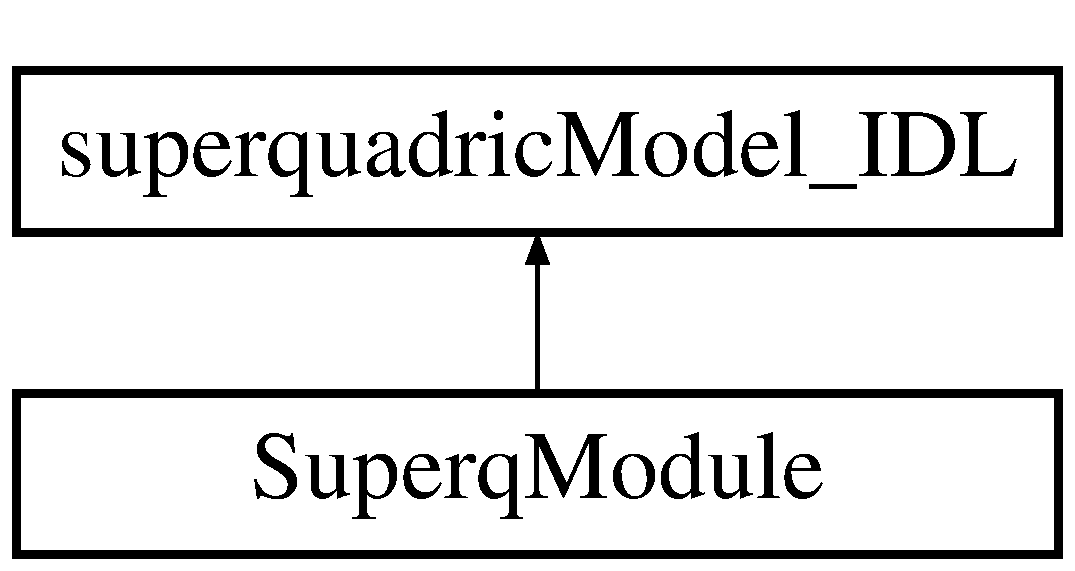
\includegraphics[height=2.000000cm]{classsuperquadricModel__IDL}
\end{center}
\end{figure}
\subsection*{Public Member Functions}
\begin{DoxyCompactItemize}
\item 
virtual bool \hyperlink{classsuperquadricModel__IDL_a781426bfc4862e87ef75a4bbbfa33275}{set\-\_\-tag\-\_\-file} (const std\-::string \&entry)
\begin{DoxyCompactList}\small\item\em Set the tag for storing files. \end{DoxyCompactList}\item 
virtual std\-::string \hyperlink{classsuperquadricModel__IDL_a6d39eaa247aec65fe2bfefbdace4ec85}{get\-\_\-tag\-\_\-file} ()
\begin{DoxyCompactList}\small\item\em Return the tag used for storing files. \end{DoxyCompactList}\item 
virtual yarp\-::os\-::\-Property \hyperlink{classsuperquadricModel__IDL_a10039bb93445066d9dd29d8f6c9ef6c5}{get\-\_\-superq} (const std\-::vector$<$ yarp\-::sig\-::\-Vector $>$ \&point\-\_\-cloud, const bool filtered\-\_\-or\-\_\-not, const bool reset\-\_\-or\-\_\-not)
\begin{DoxyCompactList}\small\item\em Get the parameters of the reconstructed superquadric. \end{DoxyCompactList}\item 
virtual bool \hyperlink{classsuperquadricModel__IDL_a1a2080d797a81b46b0dffa86b5367e15}{set\-\_\-points\-\_\-filtering} (const std\-::string \&entry)
\begin{DoxyCompactList}\small\item\em On/off point cloud filtering. \end{DoxyCompactList}\item 
virtual std\-::string \hyperlink{classsuperquadricModel__IDL_aa490ebcf39414aaaae41d5095267abb9}{get\-\_\-points\-\_\-filtering} ()
\begin{DoxyCompactList}\small\item\em Say if points filtering is on or not. \end{DoxyCompactList}\item 
virtual bool \hyperlink{classsuperquadricModel__IDL_af418edf09afd9374c5272d018c58e8a7}{set\-\_\-superq\-\_\-filtering} (const std\-::string \&entry)
\begin{DoxyCompactList}\small\item\em On/off superquadric filtering. \end{DoxyCompactList}\item 
virtual std\-::string \hyperlink{classsuperquadricModel__IDL_af99d29d42b96b8db6c90c5fd48cfb253}{get\-\_\-superq\-\_\-filtering} ()
\begin{DoxyCompactList}\small\item\em Say if superquadric filtering is on or not. \end{DoxyCompactList}\item 
virtual bool \hyperlink{classsuperquadricModel__IDL_a8368b783845a3e5ae7e0706ee5b888c0}{set\-\_\-save\-\_\-points} (const std\-::string \&entry)
\begin{DoxyCompactList}\small\item\em Set if you want to save the acquired point cloud. \end{DoxyCompactList}\item 
virtual std\-::string \hyperlink{classsuperquadricModel__IDL_a4b101fe118a1ee912468562bde0b0df4}{get\-\_\-save\-\_\-points} ()
\begin{DoxyCompactList}\small\item\em Set if you are saving the acquired point cloud. \end{DoxyCompactList}\item 
virtual yarp\-::os\-::\-Property \hyperlink{classsuperquadricModel__IDL_a50b388a29852f9d8b57a0bbb276d4675}{get\-\_\-options} (const std\-::string \&field)
\begin{DoxyCompactList}\small\item\em Get the parameters of the module. \end{DoxyCompactList}\item 
virtual bool \hyperlink{classsuperquadricModel__IDL_a575e0b591f07206b0d6c29e5cfeead37}{set\-\_\-options} (const yarp\-::os\-::\-Property \&options, const std\-::string \&field)
\begin{DoxyCompactList}\small\item\em Set the parameters of the module. \end{DoxyCompactList}\item 
virtual bool \hyperlink{classsuperquadricModel__IDL_a651c741e9b01b25d46be96b06b91011d}{set\-\_\-visualization} (const std\-::string \&e)
\begin{DoxyCompactList}\small\item\em Set if the visualization has to be enabled. \end{DoxyCompactList}\item 
virtual std\-::string \hyperlink{classsuperquadricModel__IDL_a5d9f4f0622ba19b60218636dc108ef61}{get\-\_\-visualization} ()
\begin{DoxyCompactList}\small\item\em Get if visualization is enabled. \end{DoxyCompactList}\item 
virtual bool {\bfseries read} (yarp\-::os\-::\-Connection\-Reader \&connection)\label{classsuperquadricModel__IDL_ac72a24dddca13978d7adcd5cf4f40b1f}

\item 
virtual std\-::vector$<$ std\-::string $>$ {\bfseries help} (const std\-::string \&function\-Name=\char`\"{}-\/-\/all\char`\"{})\label{classsuperquadricModel__IDL_a263ca3dc1c7a21cc3ac40caadc95cf3d}

\end{DoxyCompactItemize}


\subsection{Detailed Description}
\hyperlink{classsuperquadricModel__IDL}{superquadric\-Model\-\_\-\-I\-D\-L} I\-D\-L Interface to \hyperlink{group__superquadric-model}{superquadric-\/model} services. 

Definition at line 19 of file superquadric\-Model\-\_\-\-I\-D\-L.\-h.



\subsection{Member Function Documentation}
\index{superquadric\-Model\-\_\-\-I\-D\-L@{superquadric\-Model\-\_\-\-I\-D\-L}!get\-\_\-options@{get\-\_\-options}}
\index{get\-\_\-options@{get\-\_\-options}!superquadricModel_IDL@{superquadric\-Model\-\_\-\-I\-D\-L}}
\subsubsection[{get\-\_\-options}]{\setlength{\rightskip}{0pt plus 5cm}virtual yarp\-::os\-::\-Property superquadric\-Model\-\_\-\-I\-D\-L\-::get\-\_\-options (
\begin{DoxyParamCaption}
\item[{const std\-::string \&}]{field}
\end{DoxyParamCaption}
)\hspace{0.3cm}{\ttfamily [virtual]}}\label{classsuperquadricModel__IDL_a50b388a29852f9d8b57a0bbb276d4675}


Get the parameters of the module. 

The user must pay attention in changing them. 
\begin{DoxyParams}{Parameters}
{\em field} & can be \char`\"{}points\-\_\-filter\char`\"{}, \char`\"{}superq\-\_\-filter\char`\"{}, \char`\"{}optimization\char`\"{}, \char`\"{}visualization\char`\"{} or \char`\"{}statistics\char`\"{}. depending on which parameters we are interested in. \\
\hline
\end{DoxyParams}
\begin{DoxyReturn}{Returns}
the Property including all the parameter values. 
\end{DoxyReturn}


Reimplemented in \hyperlink{classSuperqModule_a18822e0a99dc0b13479f20960c577fb9}{Superq\-Module}.

\index{superquadric\-Model\-\_\-\-I\-D\-L@{superquadric\-Model\-\_\-\-I\-D\-L}!get\-\_\-points\-\_\-filtering@{get\-\_\-points\-\_\-filtering}}
\index{get\-\_\-points\-\_\-filtering@{get\-\_\-points\-\_\-filtering}!superquadricModel_IDL@{superquadric\-Model\-\_\-\-I\-D\-L}}
\subsubsection[{get\-\_\-points\-\_\-filtering}]{\setlength{\rightskip}{0pt plus 5cm}virtual std\-::string superquadric\-Model\-\_\-\-I\-D\-L\-::get\-\_\-points\-\_\-filtering (
\begin{DoxyParamCaption}
{}
\end{DoxyParamCaption}
)\hspace{0.3cm}{\ttfamily [virtual]}}\label{classsuperquadricModel__IDL_aa490ebcf39414aaaae41d5095267abb9}


Say if points filtering is on or not. 

\begin{DoxyReturn}{Returns}
on/off string if points filtering is on/off. 
\end{DoxyReturn}


Reimplemented in \hyperlink{classSuperqModule_a60c8ff17436cc55a3e9b704dd6c2529b}{Superq\-Module}.

\index{superquadric\-Model\-\_\-\-I\-D\-L@{superquadric\-Model\-\_\-\-I\-D\-L}!get\-\_\-save\-\_\-points@{get\-\_\-save\-\_\-points}}
\index{get\-\_\-save\-\_\-points@{get\-\_\-save\-\_\-points}!superquadricModel_IDL@{superquadric\-Model\-\_\-\-I\-D\-L}}
\subsubsection[{get\-\_\-save\-\_\-points}]{\setlength{\rightskip}{0pt plus 5cm}virtual std\-::string superquadric\-Model\-\_\-\-I\-D\-L\-::get\-\_\-save\-\_\-points (
\begin{DoxyParamCaption}
{}
\end{DoxyParamCaption}
)\hspace{0.3cm}{\ttfamily [virtual]}}\label{classsuperquadricModel__IDL_a4b101fe118a1ee912468562bde0b0df4}


Set if you are saving the acquired point cloud. 

\begin{DoxyReturn}{Returns}
\char`\"{}on\char`\"{} or \char`\"{}off\char`\"{}. 
\end{DoxyReturn}


Reimplemented in \hyperlink{classSuperqModule_adfeeea091edd0d32d388b072f4fc9d93}{Superq\-Module}.

\index{superquadric\-Model\-\_\-\-I\-D\-L@{superquadric\-Model\-\_\-\-I\-D\-L}!get\-\_\-superq@{get\-\_\-superq}}
\index{get\-\_\-superq@{get\-\_\-superq}!superquadricModel_IDL@{superquadric\-Model\-\_\-\-I\-D\-L}}
\subsubsection[{get\-\_\-superq}]{\setlength{\rightskip}{0pt plus 5cm}virtual yarp\-::os\-::\-Property superquadric\-Model\-\_\-\-I\-D\-L\-::get\-\_\-superq (
\begin{DoxyParamCaption}
\item[{const std\-::vector$<$ yarp\-::sig\-::\-Vector $>$ \&}]{point\-\_\-cloud, }
\item[{const bool}]{filtered\-\_\-or\-\_\-not, }
\item[{const bool}]{reset\-\_\-or\-\_\-not}
\end{DoxyParamCaption}
)\hspace{0.3cm}{\ttfamily [virtual]}}\label{classsuperquadricModel__IDL_a10039bb93445066d9dd29d8f6c9ef6c5}


Get the parameters of the reconstructed superquadric. 


\begin{DoxyParams}{Parameters}
{\em point\-\_\-cloud} & is the 3\-D point cloud of the object we want to model with the superquadric, for instance\-: ((100.\-0 102.\-0) (100.\-0 103.\-0) ... ). \\
\hline
{\em filtered\-\_\-or\-\_\-not} & is a bool variable specifing if we want the superquadric to be filtered (true/1) or not (false/0). \\
\hline
{\em reset\-\_\-or\-\_\-not} & is a bool variable specifing if we want to reset the superquadric filtered (if enabled) or not. \\
\hline
\end{DoxyParams}
\begin{DoxyReturn}{Returns}
the 12 parameters (x0, .. x11) of the current superquadric. In particular, the parameters are grouped in a Property as follows\-: \char`\"{}dimensions\char`\"{} (x0, x1, x2) are the three semi-\/axes lenghts; \char`\"{}exponents\char`\"{} (x3 and x4) are the exponents, responsible for the superquadric shape; \char`\"{}center\char`\"{}(x5, x6, x7) contains the coordinate of the superquadric center; and \char`\"{}orientation\char`\"{} (x8, x9, 10, x11) is the axis-\/angle representation obtained from the Euler angles. 
\end{DoxyReturn}
\index{superquadric\-Model\-\_\-\-I\-D\-L@{superquadric\-Model\-\_\-\-I\-D\-L}!get\-\_\-superq\-\_\-filtering@{get\-\_\-superq\-\_\-filtering}}
\index{get\-\_\-superq\-\_\-filtering@{get\-\_\-superq\-\_\-filtering}!superquadricModel_IDL@{superquadric\-Model\-\_\-\-I\-D\-L}}
\subsubsection[{get\-\_\-superq\-\_\-filtering}]{\setlength{\rightskip}{0pt plus 5cm}virtual std\-::string superquadric\-Model\-\_\-\-I\-D\-L\-::get\-\_\-superq\-\_\-filtering (
\begin{DoxyParamCaption}
{}
\end{DoxyParamCaption}
)\hspace{0.3cm}{\ttfamily [virtual]}}\label{classsuperquadricModel__IDL_af99d29d42b96b8db6c90c5fd48cfb253}


Say if superquadric filtering is on or not. 

\begin{DoxyReturn}{Returns}
on/off string if superquadeic filtering is on/off. 
\end{DoxyReturn}


Reimplemented in \hyperlink{classSuperqModule_a66cb1b371b92687d851b5ca23174198b}{Superq\-Module}.

\index{superquadric\-Model\-\_\-\-I\-D\-L@{superquadric\-Model\-\_\-\-I\-D\-L}!get\-\_\-tag\-\_\-file@{get\-\_\-tag\-\_\-file}}
\index{get\-\_\-tag\-\_\-file@{get\-\_\-tag\-\_\-file}!superquadricModel_IDL@{superquadric\-Model\-\_\-\-I\-D\-L}}
\subsubsection[{get\-\_\-tag\-\_\-file}]{\setlength{\rightskip}{0pt plus 5cm}virtual std\-::string superquadric\-Model\-\_\-\-I\-D\-L\-::get\-\_\-tag\-\_\-file (
\begin{DoxyParamCaption}
{}
\end{DoxyParamCaption}
)\hspace{0.3cm}{\ttfamily [virtual]}}\label{classsuperquadricModel__IDL_a6d39eaa247aec65fe2bfefbdace4ec85}


Return the tag used for storing files. 

\begin{DoxyReturn}{Returns}
the tag name. 
\end{DoxyReturn}


Reimplemented in \hyperlink{classSuperqModule_ac5475155a5a1b05e5fdef54699cef1a6}{Superq\-Module}.

\index{superquadric\-Model\-\_\-\-I\-D\-L@{superquadric\-Model\-\_\-\-I\-D\-L}!get\-\_\-visualization@{get\-\_\-visualization}}
\index{get\-\_\-visualization@{get\-\_\-visualization}!superquadricModel_IDL@{superquadric\-Model\-\_\-\-I\-D\-L}}
\subsubsection[{get\-\_\-visualization}]{\setlength{\rightskip}{0pt plus 5cm}virtual std\-::string superquadric\-Model\-\_\-\-I\-D\-L\-::get\-\_\-visualization (
\begin{DoxyParamCaption}
{}
\end{DoxyParamCaption}
)\hspace{0.3cm}{\ttfamily [virtual]}}\label{classsuperquadricModel__IDL_a5d9f4f0622ba19b60218636dc108ef61}


Get if visualization is enabled. 

\begin{DoxyReturn}{Returns}
\char`\"{}on\char`\"{} or \char`\"{}off\char`\"{}. 
\end{DoxyReturn}


Reimplemented in \hyperlink{classSuperqModule_a89be4778051c4dd19339021448f89b41}{Superq\-Module}.

\index{superquadric\-Model\-\_\-\-I\-D\-L@{superquadric\-Model\-\_\-\-I\-D\-L}!set\-\_\-options@{set\-\_\-options}}
\index{set\-\_\-options@{set\-\_\-options}!superquadricModel_IDL@{superquadric\-Model\-\_\-\-I\-D\-L}}
\subsubsection[{set\-\_\-options}]{\setlength{\rightskip}{0pt plus 5cm}virtual bool superquadric\-Model\-\_\-\-I\-D\-L\-::set\-\_\-options (
\begin{DoxyParamCaption}
\item[{const yarp\-::os\-::\-Property \&}]{options, }
\item[{const std\-::string \&}]{field}
\end{DoxyParamCaption}
)\hspace{0.3cm}{\ttfamily [virtual]}}\label{classsuperquadricModel__IDL_a575e0b591f07206b0d6c29e5cfeead37}


Set the parameters of the module. 

The user must pay attention in changing them. 
\begin{DoxyParams}{Parameters}
{\em options} & is a Property containing the parameters the user want to change. \\
\hline
{\em field} & is a string specifying which can of parameter we are going to change. Field can be\-: \char`\"{}points\-\_\-filter\char`\"{}, \char`\"{}superq\-\_\-filter\char`\"{}, \char`\"{}optimization\char`\"{} or \char`\"{}visualization\char`\"{}. You can set the parameters typing\-: command\-: set\-\_\-options ((filter\-\_\-radius $<$radius-\/value$>$) (filter\-\_\-nn\-Threshold $<$nn\-Threshold-\/value$>$)) points\-\_\-filter. \\
\hline
\end{DoxyParams}
\begin{DoxyReturn}{Returns}
true/false on success/failure. 
\end{DoxyReturn}


Reimplemented in \hyperlink{classSuperqModule_a32ccf59ac0572ca77883237dd2d12890}{Superq\-Module}.

\index{superquadric\-Model\-\_\-\-I\-D\-L@{superquadric\-Model\-\_\-\-I\-D\-L}!set\-\_\-points\-\_\-filtering@{set\-\_\-points\-\_\-filtering}}
\index{set\-\_\-points\-\_\-filtering@{set\-\_\-points\-\_\-filtering}!superquadricModel_IDL@{superquadric\-Model\-\_\-\-I\-D\-L}}
\subsubsection[{set\-\_\-points\-\_\-filtering}]{\setlength{\rightskip}{0pt plus 5cm}virtual bool superquadric\-Model\-\_\-\-I\-D\-L\-::set\-\_\-points\-\_\-filtering (
\begin{DoxyParamCaption}
\item[{const std\-::string \&}]{entry}
\end{DoxyParamCaption}
)\hspace{0.3cm}{\ttfamily [virtual]}}\label{classsuperquadricModel__IDL_a1a2080d797a81b46b0dffa86b5367e15}


On/off point cloud filtering. 


\begin{DoxyParams}{Parameters}
{\em entry} & is \char`\"{}on/off\char`\"{} if you want/do not want to filter points. \\
\hline
\end{DoxyParams}
\begin{DoxyReturn}{Returns}
true/false on success/failure. 
\end{DoxyReturn}


Reimplemented in \hyperlink{classSuperqModule_a408203d0119443fb61544f84dafff8a4}{Superq\-Module}.

\index{superquadric\-Model\-\_\-\-I\-D\-L@{superquadric\-Model\-\_\-\-I\-D\-L}!set\-\_\-save\-\_\-points@{set\-\_\-save\-\_\-points}}
\index{set\-\_\-save\-\_\-points@{set\-\_\-save\-\_\-points}!superquadricModel_IDL@{superquadric\-Model\-\_\-\-I\-D\-L}}
\subsubsection[{set\-\_\-save\-\_\-points}]{\setlength{\rightskip}{0pt plus 5cm}virtual bool superquadric\-Model\-\_\-\-I\-D\-L\-::set\-\_\-save\-\_\-points (
\begin{DoxyParamCaption}
\item[{const std\-::string \&}]{entry}
\end{DoxyParamCaption}
)\hspace{0.3cm}{\ttfamily [virtual]}}\label{classsuperquadricModel__IDL_a8368b783845a3e5ae7e0706ee5b888c0}


Set if you want to save the acquired point cloud. 


\begin{DoxyParams}{Parameters}
{\em entry} & can be\-: \char`\"{}on\char`\"{} or \char`\"{}off\char`\"{}. \\
\hline
\end{DoxyParams}
\begin{DoxyReturn}{Returns}
true/false on success/failure. 
\end{DoxyReturn}


Reimplemented in \hyperlink{classSuperqModule_a90826fc53859ecf126f22a2569611b2c}{Superq\-Module}.

\index{superquadric\-Model\-\_\-\-I\-D\-L@{superquadric\-Model\-\_\-\-I\-D\-L}!set\-\_\-superq\-\_\-filtering@{set\-\_\-superq\-\_\-filtering}}
\index{set\-\_\-superq\-\_\-filtering@{set\-\_\-superq\-\_\-filtering}!superquadricModel_IDL@{superquadric\-Model\-\_\-\-I\-D\-L}}
\subsubsection[{set\-\_\-superq\-\_\-filtering}]{\setlength{\rightskip}{0pt plus 5cm}virtual bool superquadric\-Model\-\_\-\-I\-D\-L\-::set\-\_\-superq\-\_\-filtering (
\begin{DoxyParamCaption}
\item[{const std\-::string \&}]{entry}
\end{DoxyParamCaption}
)\hspace{0.3cm}{\ttfamily [virtual]}}\label{classsuperquadricModel__IDL_af418edf09afd9374c5272d018c58e8a7}


On/off superquadric filtering. 


\begin{DoxyParams}{Parameters}
{\em entry} & is \char`\"{}on/off\char`\"{} if you want/do not want to filter the estimated superquadric. \\
\hline
\end{DoxyParams}
\begin{DoxyReturn}{Returns}
true/false on success/failure. 
\end{DoxyReturn}


Reimplemented in \hyperlink{classSuperqModule_a902d4a48d1a919ff9d9b1f7d1c132577}{Superq\-Module}.

\index{superquadric\-Model\-\_\-\-I\-D\-L@{superquadric\-Model\-\_\-\-I\-D\-L}!set\-\_\-tag\-\_\-file@{set\-\_\-tag\-\_\-file}}
\index{set\-\_\-tag\-\_\-file@{set\-\_\-tag\-\_\-file}!superquadricModel_IDL@{superquadric\-Model\-\_\-\-I\-D\-L}}
\subsubsection[{set\-\_\-tag\-\_\-file}]{\setlength{\rightskip}{0pt plus 5cm}virtual bool superquadric\-Model\-\_\-\-I\-D\-L\-::set\-\_\-tag\-\_\-file (
\begin{DoxyParamCaption}
\item[{const std\-::string \&}]{entry}
\end{DoxyParamCaption}
)\hspace{0.3cm}{\ttfamily [virtual]}}\label{classsuperquadricModel__IDL_a781426bfc4862e87ef75a4bbbfa33275}


Set the tag for storing files. 


\begin{DoxyParams}{Parameters}
{\em entry} & is the tag that will be used in file names. \\
\hline
\end{DoxyParams}
\begin{DoxyReturn}{Returns}
true. 
\end{DoxyReturn}


Reimplemented in \hyperlink{classSuperqModule_ae9f0cfead2c367e4c3aa25292b5c42c6}{Superq\-Module}.

\index{superquadric\-Model\-\_\-\-I\-D\-L@{superquadric\-Model\-\_\-\-I\-D\-L}!set\-\_\-visualization@{set\-\_\-visualization}}
\index{set\-\_\-visualization@{set\-\_\-visualization}!superquadricModel_IDL@{superquadric\-Model\-\_\-\-I\-D\-L}}
\subsubsection[{set\-\_\-visualization}]{\setlength{\rightskip}{0pt plus 5cm}virtual bool superquadric\-Model\-\_\-\-I\-D\-L\-::set\-\_\-visualization (
\begin{DoxyParamCaption}
\item[{const std\-::string \&}]{e}
\end{DoxyParamCaption}
)\hspace{0.3cm}{\ttfamily [virtual]}}\label{classsuperquadricModel__IDL_a651c741e9b01b25d46be96b06b91011d}


Set if the visualization has to be enabled. 

\begin{DoxyReturn}{Returns}
true/false on success/failure. 
\end{DoxyReturn}


Reimplemented in \hyperlink{classSuperqModule_ae4fc54ad89b3ee72ab5ea8c8b5065866}{Superq\-Module}.



The documentation for this class was generated from the following file\-:\begin{DoxyCompactItemize}
\item 
/home/gvezzani/\-Desktop/\-Ph\-D/\-Anno\-\_\-1/super\-Quadratiche/superquadric-\/model/idl\-\_\-dox/superquadric\-Model\-\_\-\-I\-D\-L.\-h\end{DoxyCompactItemize}

\section{Superq\-Visualization Class Reference}
\label{classSuperqVisualization}\index{Superq\-Visualization@{Superq\-Visualization}}


This class shows the point cloud used for modeling or the estimated superquadric overlapped on the camera image and in real time.  




{\ttfamily \#include $<$superq\-Visualization.\-h$>$}



Inherits Rate\-Thread.

\subsection*{Public Member Functions}
\begin{DoxyCompactItemize}
\item 
{\bfseries Superq\-Visualization} (int rate, const std\-::string \&\-\_\-eye, const std\-::string \&\-\_\-what\-\_\-to\-\_\-plot, yarp\-::sig\-::\-Vector \&x, yarp\-::sig\-::\-Vector \&x\-\_\-filtered, std\-::deque$<$ int $>$ \&\-\_\-\-Color, yarp\-::dev\-::\-I\-Gaze\-Control $\ast$\-\_\-igaze, const yarp\-::sig\-::\-Matrix \-\_\-\-K, std\-::deque$<$ yarp\-::sig\-::\-Vector $>$ \&\-\_\-points, const int \&\-\_\-vis\-\_\-points, const int \&\-\_\-vis\-\_\-step, yarp\-::sig\-::\-Image\-Of$<$ yarp\-::sig\-::\-Pixel\-Rgb $>$ $\ast$\&\hyperlink{classSuperqVisualization_a884771e5af001207eb1ba6e9ac15f8a1}{img\-In})\label{classSuperqVisualization_ae6d66a2ecd9c3d544c930e67f89d7d61}

\item 
bool \hyperlink{classSuperqVisualization_aea374f59e3b941e688c1ddafad8896b9}{show\-Points} ()
\begin{DoxyCompactList}\small\item\em Show point cloud on the image. \end{DoxyCompactList}\item 
bool \hyperlink{classSuperqVisualization_aa763f8f73c82d4de1d47b03ae9d2e276}{show\-Superq} (yarp\-::sig\-::\-Vector \&x\-\_\-to\-\_\-show)
\begin{DoxyCompactList}\small\item\em Show reconstructed superquadric on the image. \end{DoxyCompactList}\item 
yarp\-::sig\-::\-Vector \hyperlink{classSuperqVisualization_aff405a4d0ad916decad09f923e319be6}{from3\-Dto2\-D} (const yarp\-::sig\-::\-Vector \&point3\-D)
\begin{DoxyCompactList}\small\item\em Compute 2\-D pixels from 3\-D points. \end{DoxyCompactList}\item 
virtual bool \hyperlink{classSuperqVisualization_a93dc1583d46a71bbcc4e4ef7f65820b9}{thread\-Init} ()\label{classSuperqVisualization_a93dc1583d46a71bbcc4e4ef7f65820b9}

\begin{DoxyCompactList}\small\item\em Init function of Rate\-Thread. \end{DoxyCompactList}\item 
virtual void \hyperlink{classSuperqVisualization_a46d689c65cec6c04d3fffdbfbbd1838b}{run} ()\label{classSuperqVisualization_a46d689c65cec6c04d3fffdbfbbd1838b}

\begin{DoxyCompactList}\small\item\em Run function of Rate\-Thread. \end{DoxyCompactList}\item 
virtual void \hyperlink{classSuperqVisualization_ae79d791d2accf581cbe0502d579f5416}{thread\-Release} ()\label{classSuperqVisualization_ae79d791d2accf581cbe0502d579f5416}

\begin{DoxyCompactList}\small\item\em Release function of Rate\-Thread. \end{DoxyCompactList}\item 
void \hyperlink{classSuperqVisualization_acbc374ffecb809ca16853c9475d7f347}{set\-Par} (const std\-::string \&par\-\_\-name, const std\-::string \&value)
\begin{DoxyCompactList}\small\item\em Set a given parameter equal to a string. \end{DoxyCompactList}\item 
void \hyperlink{classSuperqVisualization_a2403b8fcb9448e61866fd39035a482f0}{set\-Par} (const std\-::string \&par\-\_\-name, const int \&value)
\begin{DoxyCompactList}\small\item\em Set a given parameter equal to a desired value. \end{DoxyCompactList}\item 
void \hyperlink{classSuperqVisualization_a82eb6b92c07720b35c714a3c8e2f88a3}{set\-Color} (const int \&r, const int \&g, const int \&b)
\begin{DoxyCompactList}\small\item\em Set color for visualization. \end{DoxyCompactList}\item 
void \hyperlink{classSuperqVisualization_a5250a90e5865bf45c0bd8ae919b8eab0}{set\-Par} (const yarp\-::os\-::\-Property \&new\-Options, bool first\-\_\-time)
\begin{DoxyCompactList}\small\item\em Set parameters for visualization. \end{DoxyCompactList}\item 
yarp\-::os\-::\-Property \hyperlink{classSuperqVisualization_ae4fac8f79629a3fa81a688ab4baf61f7}{get\-Par} ()
\begin{DoxyCompactList}\small\item\em Get parameters for visualization. \end{DoxyCompactList}\item 
double \hyperlink{classSuperqVisualization_a9583b378f68f466a76022817d3051c6e}{get\-Time} ()
\begin{DoxyCompactList}\small\item\em Get time required for visualization. \end{DoxyCompactList}\end{DoxyCompactItemize}
\subsection*{Data Fields}
\begin{DoxyCompactItemize}
\item 
yarp\-::sig\-::\-Vector \& \hyperlink{classSuperqVisualization_a57358b13afc9b5aa3920b7c96b20b26d}{superq}\label{classSuperqVisualization_a57358b13afc9b5aa3920b7c96b20b26d}

\begin{DoxyCompactList}\small\item\em Estimated superquadric. \end{DoxyCompactList}\item 
yarp\-::sig\-::\-Vector \& \hyperlink{classSuperqVisualization_aed6197ba510529ed07d32a1a86a48e83}{superq\-\_\-filtered}\label{classSuperqVisualization_aed6197ba510529ed07d32a1a86a48e83}

\begin{DoxyCompactList}\small\item\em Filtered superquadric. \end{DoxyCompactList}\item 
std\-::deque$<$ yarp\-::sig\-::\-Vector $>$ \& \hyperlink{classSuperqVisualization_aa00fb7590a7bc410387e041fbdfb162a}{points}\label{classSuperqVisualization_aa00fb7590a7bc410387e041fbdfb162a}

\begin{DoxyCompactList}\small\item\em Object point cloud. \end{DoxyCompactList}\item 
yarp\-::sig\-::\-Image\-Of\\*
$<$ yarp\-::sig\-::\-Pixel\-Rgb $>$ $\ast$\& \hyperlink{classSuperqVisualization_a884771e5af001207eb1ba6e9ac15f8a1}{img\-In}\label{classSuperqVisualization_a884771e5af001207eb1ba6e9ac15f8a1}

\begin{DoxyCompactList}\small\item\em Input image. \end{DoxyCompactList}\end{DoxyCompactItemize}
\subsection*{Protected Attributes}
\begin{DoxyCompactItemize}
\item 
yarp\-::os\-::\-Buffered\-Port\\*
$<$ yarp\-::sig\-::\-Image\-Of\\*
$<$ yarp\-::sig\-::\-Pixel\-Rgb $>$ $>$ {\bfseries port\-Img\-Out}\label{classSuperqVisualization_a0ed5bf82e324579e781952b7a540d5c0}

\item 
int {\bfseries r}\label{classSuperqVisualization_aee081a694340a9a8658a960872cb6172}

\item 
int {\bfseries g}\label{classSuperqVisualization_a51cc6e3ac3ee243250a7042f00c813d1}

\item 
int {\bfseries b}\label{classSuperqVisualization_a96c39287f863466bbbc21342dd62b68a}

\item 
double {\bfseries t\-\_\-vis}\label{classSuperqVisualization_af984de33154bf4ebe0abf6f1f5047a1c}

\item 
int {\bfseries vis\-\_\-step}\label{classSuperqVisualization_a43a34e1d587532fbff246941cd28e3b6}

\item 
int {\bfseries vis\-\_\-points}\label{classSuperqVisualization_a97eaa294a7c48033ef5695976556435a}

\item 
std\-::string {\bfseries what\-\_\-to\-\_\-plot}\label{classSuperqVisualization_a60f1dd2489b897777edffc4dfdebe64d}

\item 
yarp\-::sig\-::\-Vector {\bfseries point}\label{classSuperqVisualization_a77fbae5c4996f393cae867d56cf2ee16}

\item 
yarp\-::sig\-::\-Vector {\bfseries point1}\label{classSuperqVisualization_a43a15830ead614d6962ac4777c8fc014}

\item 
yarp\-::sig\-::\-Vector {\bfseries point2\-D}\label{classSuperqVisualization_a186ba8f98b1344934bab2fc2de516375}

\item 
std\-::deque$<$ int $>$ {\bfseries Color}\label{classSuperqVisualization_ae976f619addaebdf724316f25e2c38a8}

\item 
std\-::string {\bfseries eye}\label{classSuperqVisualization_a57cd2c0f68d9bf7365b8c9334b7c07bd}

\item 
yarp\-::sig\-::\-Matrix {\bfseries R}\label{classSuperqVisualization_ad38ada4dfaaf6ced81c6da9aacba4bc0}

\item 
yarp\-::sig\-::\-Matrix {\bfseries H}\label{classSuperqVisualization_a64d02e9b2b003bb30235522f1b293a59}

\item 
yarp\-::sig\-::\-Matrix {\bfseries K}\label{classSuperqVisualization_a3b44b49611b760f95341303143b72804}

\item 
yarp\-::dev\-::\-I\-Gaze\-Control $\ast$ {\bfseries igaze}\label{classSuperqVisualization_a70393943f451663a458119c63b6e0ebf}

\item 
yarp\-::os\-::\-Mutex {\bfseries mutex}\label{classSuperqVisualization_a5925440ac066d2d7dd40df5758e76bbf}

\end{DoxyCompactItemize}


\subsection{Detailed Description}
This class shows the point cloud used for modeling or the estimated superquadric overlapped on the camera image and in real time. 

Definition at line 36 of file superq\-Visualization.\-h.



\subsection{Member Function Documentation}
\index{Superq\-Visualization@{Superq\-Visualization}!from3\-Dto2\-D@{from3\-Dto2\-D}}
\index{from3\-Dto2\-D@{from3\-Dto2\-D}!SuperqVisualization@{Superq\-Visualization}}
\subsubsection[{from3\-Dto2\-D}]{\setlength{\rightskip}{0pt plus 5cm}Vector Superq\-Visualization\-::from3\-Dto2\-D (
\begin{DoxyParamCaption}
\item[{const yarp\-::sig\-::\-Vector \&}]{point3\-D}
\end{DoxyParamCaption}
)}\label{classSuperqVisualization_aff405a4d0ad916decad09f923e319be6}


Compute 2\-D pixels from 3\-D points. 


\begin{DoxyParams}{Parameters}
{\em point3\-D} & is the 3\-D point to be converted \\
\hline
\end{DoxyParams}
\begin{DoxyReturn}{Returns}
a 2\-D vector representing the corresponding pixel 
\end{DoxyReturn}


Definition at line 168 of file superq\-Visualization.\-cpp.



Referenced by show\-Points(), and show\-Superq().


\begin{DoxyCode}
169 \{
170     Vector point2D(3,0.0);
171     Vector point\_aux(4,1.0);
172     point\_aux.setSubvector(0,point3D);
173     point2D=K*H*point\_aux;
174     \textcolor{keywordflow}{return} point2D.subVector(0,1)/point2D[2];
175 \}
\end{DoxyCode}
\index{Superq\-Visualization@{Superq\-Visualization}!get\-Par@{get\-Par}}
\index{get\-Par@{get\-Par}!SuperqVisualization@{Superq\-Visualization}}
\subsubsection[{get\-Par}]{\setlength{\rightskip}{0pt plus 5cm}Property Superq\-Visualization\-::get\-Par (
\begin{DoxyParamCaption}
{}
\end{DoxyParamCaption}
)}\label{classSuperqVisualization_ae4fac8f79629a3fa81a688ab4baf61f7}


Get parameters for visualization. 

\begin{DoxyReturn}{Returns}
a property with all the visualization options 
\end{DoxyReturn}


Definition at line 318 of file superq\-Visualization.\-cpp.


\begin{DoxyCode}
319 \{
320     LockGuard lg(mutex);
321 
322     Property advOptions;
323     advOptions.put(\textcolor{stringliteral}{"visualized\_points"},vis\_points);
324     \textcolor{keywordflow}{if} (Color[0]==255 && Color[1]==0 && Color[2]==0)
325         advOptions.put(\textcolor{stringliteral}{"color"},\textcolor{stringliteral}{"red"});
326     \textcolor{keywordflow}{else} \textcolor{keywordflow}{if}  (Color[0]==0 && Color[1]==255 && Color[2]==0)
327         advOptions.put(\textcolor{stringliteral}{"color"},\textcolor{stringliteral}{"green"});
328     \textcolor{keywordflow}{else} \textcolor{keywordflow}{if}  (Color[0]==0 && Color[1]==0 &&Color[2]==255)
329         advOptions.put(\textcolor{stringliteral}{"color"},\textcolor{stringliteral}{"blue"});
330     advOptions.put(\textcolor{stringliteral}{"camera"},eye);
331     advOptions.put(\textcolor{stringliteral}{"visualized\_points\_step"},vis\_step);
332     advOptions.put(\textcolor{stringliteral}{"what\_to\_plot"},what\_to\_plot);
333     \textcolor{keywordflow}{return} advOptions;
334 \}
\end{DoxyCode}
\index{Superq\-Visualization@{Superq\-Visualization}!get\-Time@{get\-Time}}
\index{get\-Time@{get\-Time}!SuperqVisualization@{Superq\-Visualization}}
\subsubsection[{get\-Time}]{\setlength{\rightskip}{0pt plus 5cm}double Superq\-Visualization\-::get\-Time (
\begin{DoxyParamCaption}
{}
\end{DoxyParamCaption}
)}\label{classSuperqVisualization_a9583b378f68f466a76022817d3051c6e}


Get time required for visualization. 

\begin{DoxyReturn}{Returns}
the visualization time 
\end{DoxyReturn}


Definition at line 337 of file superq\-Visualization.\-cpp.


\begin{DoxyCode}
338 \{   
339     LockGuard lg(mutex);
340     \textcolor{keywordflow}{return} t\_vis;
341 \}
\end{DoxyCode}
\index{Superq\-Visualization@{Superq\-Visualization}!set\-Color@{set\-Color}}
\index{set\-Color@{set\-Color}!SuperqVisualization@{Superq\-Visualization}}
\subsubsection[{set\-Color}]{\setlength{\rightskip}{0pt plus 5cm}void Superq\-Visualization\-::set\-Color (
\begin{DoxyParamCaption}
\item[{const int \&}]{r, }
\item[{const int \&}]{g, }
\item[{const int \&}]{b}
\end{DoxyParamCaption}
)}\label{classSuperqVisualization_a82eb6b92c07720b35c714a3c8e2f88a3}


Set color for visualization. 


\begin{DoxyParams}{Parameters}
{\em r} & is the red component \\
\hline
{\em g} & is the green component \\
\hline
{\em b} & is the blue component \\
\hline
\end{DoxyParams}
\index{Superq\-Visualization@{Superq\-Visualization}!set\-Par@{set\-Par}}
\index{set\-Par@{set\-Par}!SuperqVisualization@{Superq\-Visualization}}
\subsubsection[{set\-Par}]{\setlength{\rightskip}{0pt plus 5cm}void Superq\-Visualization\-::set\-Par (
\begin{DoxyParamCaption}
\item[{const std\-::string \&}]{par\-\_\-name, }
\item[{const std\-::string \&}]{value}
\end{DoxyParamCaption}
)}\label{classSuperqVisualization_acbc374ffecb809ca16853c9475d7f347}


Set a given parameter equal to a string. 


\begin{DoxyParams}{Parameters}
{\em par\-\_\-name} & is the name of the parameter to be changed \\
\hline
{\em value} & is the new value \\
\hline
\end{DoxyParams}
\index{Superq\-Visualization@{Superq\-Visualization}!set\-Par@{set\-Par}}
\index{set\-Par@{set\-Par}!SuperqVisualization@{Superq\-Visualization}}
\subsubsection[{set\-Par}]{\setlength{\rightskip}{0pt plus 5cm}void Superq\-Visualization\-::set\-Par (
\begin{DoxyParamCaption}
\item[{const std\-::string \&}]{par\-\_\-name, }
\item[{const int \&}]{value}
\end{DoxyParamCaption}
)}\label{classSuperqVisualization_a2403b8fcb9448e61866fd39035a482f0}


Set a given parameter equal to a desired value. 


\begin{DoxyParams}{Parameters}
{\em par\-\_\-name} & is the name of the parameter to be changed \\
\hline
{\em value} & is the new value \\
\hline
\end{DoxyParams}
\index{Superq\-Visualization@{Superq\-Visualization}!set\-Par@{set\-Par}}
\index{set\-Par@{set\-Par}!SuperqVisualization@{Superq\-Visualization}}
\subsubsection[{set\-Par}]{\setlength{\rightskip}{0pt plus 5cm}void Superq\-Visualization\-::set\-Par (
\begin{DoxyParamCaption}
\item[{const yarp\-::os\-::\-Property \&}]{new\-Options, }
\item[{bool}]{first\-\_\-time}
\end{DoxyParamCaption}
)}\label{classSuperqVisualization_a5250a90e5865bf45c0bd8ae919b8eab0}


Set parameters for visualization. 


\begin{DoxyParams}{Parameters}
{\em new\-Options} & is a Property with the new options to set \\
\hline
{\em first\-\_\-time} & takes into account if the options have already been set or not \\
\hline
\end{DoxyParams}
\index{Superq\-Visualization@{Superq\-Visualization}!show\-Points@{show\-Points}}
\index{show\-Points@{show\-Points}!SuperqVisualization@{Superq\-Visualization}}
\subsubsection[{show\-Points}]{\setlength{\rightskip}{0pt plus 5cm}bool Superq\-Visualization\-::show\-Points (
\begin{DoxyParamCaption}
{}
\end{DoxyParamCaption}
)}\label{classSuperqVisualization_aea374f59e3b941e688c1ddafad8896b9}


Show point cloud on the image. 

\begin{DoxyReturn}{Returns}
true 
\end{DoxyReturn}


Definition at line 117 of file superq\-Visualization.\-cpp.



References from3\-Dto2\-D(), img\-In, and points.



Referenced by run().


\begin{DoxyCode}
118 \{
119     PixelRgb color(Color[0],Color[1],Color[2]);
120     Stamp *stamp=NULL;
121     Vector pos, orient;
122 
123     ImageOf<PixelRgb> &imgOut=portImgOut.prepare();
124     imgOut=*imgIn;
125 
126     \textcolor{keywordflow}{if} (eye==\textcolor{stringliteral}{"left"})
127     \{
128         \textcolor{keywordflow}{if} (igaze->getLeftEyePose(pos,orient,stamp))
129         \{
130             H=axis2dcm(orient);
131             H.setSubcol(pos,0,3);
132             H=SE3inv(H);
133         \}
134     \}
135     \textcolor{keywordflow}{else}
136     \{
137         \textcolor{keywordflow}{if} (igaze->getRightEyePose(pos,orient,stamp))
138         \{
139             H=axis2dcm(orient);
140             H.setSubcol(pos,0,3);
141             H=SE3inv(H);
142         \}
143     \}
144 
145     Vector point(3,0.0);
146 
147      \textcolor{keywordflow}{for} (\textcolor{keywordtype}{size\_t} i=0; i<points.size(); i+=vis\_step)
148      \{
149          point=points[i].subVector(0,2);
150          point2D=from3Dto2D(point);
151 
152          cv::Point target\_point((\textcolor{keywordtype}{int})point2D[0],(\textcolor{keywordtype}{int})point2D[1]);
153 
154          \textcolor{keywordflow}{if} ((target\_point.x<0) || (target\_point.y<0) || (target\_point.x>=320) || (target\_point.y>=240))
155          \{
156              yWarning(\textcolor{stringliteral}{"[SuperqVisualization]:  Not acceptable pixels!"});
157          \}
158          \textcolor{keywordflow}{else}
159             imgOut.pixel(target\_point.x, target\_point.y)=color;
160      \}
161 
162     portImgOut.write();
163 
164     \textcolor{keywordflow}{return} \textcolor{keyword}{true};
165 \}
\end{DoxyCode}
\index{Superq\-Visualization@{Superq\-Visualization}!show\-Superq@{show\-Superq}}
\index{show\-Superq@{show\-Superq}!SuperqVisualization@{Superq\-Visualization}}
\subsubsection[{show\-Superq}]{\setlength{\rightskip}{0pt plus 5cm}bool Superq\-Visualization\-::show\-Superq (
\begin{DoxyParamCaption}
\item[{yarp\-::sig\-::\-Vector \&}]{x\-\_\-to\-\_\-show}
\end{DoxyParamCaption}
)}\label{classSuperqVisualization_aa763f8f73c82d4de1d47b03ae9d2e276}


Show reconstructed superquadric on the image. 


\begin{DoxyParams}{Parameters}
{\em x\-\_\-to\-\_\-show} & is the superquadric to be shown \\
\hline
\end{DoxyParams}
\begin{DoxyReturn}{Returns}
true/false on success/failure 
\end{DoxyReturn}


Definition at line 39 of file superq\-Visualization.\-cpp.



References from3\-Dto2\-D(), and img\-In.



Referenced by run().


\begin{DoxyCode}
40 \{
41     LockGuard lg(mutex);
42 
43     PixelRgb color(Color[0],Color[1],Color[2]);
44     Vector pos, orient;
45     \textcolor{keywordtype}{double} co,so,ce,se;
46     Stamp *stamp=NULL;
47 
48     ImageOf<PixelRgb> &imgOut=portImgOut.prepare();
49     imgOut=*imgIn;
50 
51     R=euler2dcm(x\_toshow.subVector(8,10));
52     R=R.transposed();
53 
54     \textcolor{keywordflow}{if} ((norm(x\_toshow)>0.0))
55     \{
56         \textcolor{keywordflow}{if} (eye==\textcolor{stringliteral}{"left"})
57         \{
58             \textcolor{keywordflow}{if} (igaze->getLeftEyePose(pos,orient,stamp))
59             \{
60                 H=axis2dcm(orient);
61                 H.setSubcol(pos,0,3);
62                 H=SE3inv(H);
63             \}
64         \}
65         \textcolor{keywordflow}{else}
66         \{
67             \textcolor{keywordflow}{if} (igaze->getRightEyePose(pos,orient,stamp))
68             \{
69                 H=axis2dcm(orient);
70                 H.setSubcol(pos,0,3);
71                 H=SE3inv(H);
72             \}
73         \}
74 
75         \textcolor{keywordtype}{double} step=2*M\_PI/vis\_points;
76 
77         \textcolor{keywordflow}{for} (\textcolor{keywordtype}{double} eta=-M\_PI; eta<M\_PI; eta+=step)
78         \{
79              \textcolor{keywordflow}{for} (\textcolor{keywordtype}{double} omega=-M\_PI; omega<M\_PI;omega+=step)
80              \{
81                  co=cos(omega); so=sin(omega);
82                  ce=cos(eta); se=sin(eta);
83 
84                  point[0]=x\_toshow[0] * sign(ce)*(pow(abs(ce),x\_toshow[3])) * sign(co)*(pow(abs(co),
      x\_toshow[4])) * R(0,0) +
85                             x\_toshow[1] * sign(ce)*(pow(abs(ce),x\_toshow[3]))* sign(so)*(pow(abs(so),
      x\_toshow[4])) * R(0,1)+
86                                 x\_toshow[2] * sign(se)*(pow(abs(se),x\_toshow[3])) * R(0,2) + x\_toshow[5];
87 
88                  point[1]=x\_toshow[0] * sign(ce)*(pow(abs(ce),x\_toshow[3])) * sign(co)*(pow(abs(co),
      x\_toshow[4])) * R(1,0) +
89                             x\_toshow[1] * sign(ce)*(pow(abs(ce),x\_toshow[3])) * sign(so)*(pow(abs(so),
      x\_toshow[4])) * R(1,1)+
90                                 x\_toshow[2] * sign(se)*(pow(abs(se),x\_toshow[3])) * R(1,2) + x\_toshow[6];
91 
92                  point[2]=x\_toshow[0] * sign(ce)*(pow(abs(ce),x\_toshow[3])) * sign(co)*(pow(abs(co),
      x\_toshow[4])) * R(2,0) +
93                             x\_toshow[1] * sign(ce)*(pow(abs(ce),x\_toshow[3])) * sign(so)*(pow(abs(so),
      x\_toshow[4])) * R(2,1)+
94                                 x\_toshow[2] * sign(se)*(pow(abs(se),x\_toshow[3])) * R(2,2) + x\_toshow[7];
95 
96                  point2D=from3Dto2D(point);
97 
98                  cv::Point target\_point((\textcolor{keywordtype}{int})point2D[0],(\textcolor{keywordtype}{int})point2D[1]);
99 
100                  \textcolor{keywordflow}{if} ((target\_point.x<0) || (target\_point.y<0) || (target\_point.x>=320) || (target\_point.y>=
      240))
101                  \{
102                      yWarning(\textcolor{stringliteral}{"[SuperqVisualization]: Not acceptable pixels!"});
103                  \}
104                  \textcolor{keywordflow}{else}
105                     imgOut.pixel(target\_point.x, target\_point.y)=color;
106              \}
107          \}
108     \}
109 
110     portImgOut.write();
111 
112     \textcolor{keywordflow}{return} \textcolor{keyword}{true};
113 
114 \}
\end{DoxyCode}


The documentation for this class was generated from the following files\-:\begin{DoxyCompactItemize}
\item 
/home/gvezzani/\-Desktop/\-Ph\-D/\-Anno\-\_\-1/super\-Quadratiche/superquadric-\/model/include/superq\-Visualization.\-h\item 
/home/gvezzani/\-Desktop/\-Ph\-D/\-Anno\-\_\-1/super\-Quadratiche/superquadric-\/model/src/superq\-Visualization.\-cpp\end{DoxyCompactItemize}

%--- End generated contents ---

% Index
\newpage
\phantomsection
\addcontentsline{toc}{chapter}{Index}
\printindex

\end{document}
